%%%%%%%%%%%%%%%%%%%%%%%%%%%%%%%%%%%%%%%%%%%%%%%%%%%%%%%%%%%%%%%%%%%%%%
% Overleaf (WriteLaTeX) Example: Molecular Chemistry Presentation
%
% Source: http://www.overleaf.com
%
% In these slides we show how Overleaf can be used with standard 
% chemistry packages to easily create professional presentations.
% 
% Feel free to distribute this example, but please keep the referral
% to overleaf.com
% 
%%%%%%%%%%%%%%%%%%%%%%%%%%%%%%%%%%%%%%%%%%%%%%%%%%%%%%%%%%%%%%%%%%%%%%

\documentclass[xcolor={dvipsnames}]{beamer}

\mode<presentation>
{
  \usetheme{Madrid}       % or try default, Darmstadt, Warsaw, ...
  \usecolortheme{default} % or try albatross, beaver, crane, ...
  \usefonttheme{default}    % or try default, structurebold, ...
  \setbeamertemplate{navigation symbols}{}
  \setbeamertemplate{caption}[numbered]
} 

\usepackage[english]{babel}
\usepackage[utf8x]{inputenc}
\usepackage{graphicx}
\usepackage{hyperref}
  \hypersetup{colorlinks=true}
  \hypersetup{urlcolor=blue}
  \hypersetup{linkcolor = .}
\usepackage{xcolor}
\usepackage{siunitx}
  \sisetup{separate-uncertainty = true}
\usepackage{physics}
\usepackage[font=small,labelfont=bf]{caption}
\usepackage{subcaption}
\usepackage[en-GB]{datetime2}
\usepackage{overpic}
\usepackage{feynmp}
\DeclareGraphicsRule{*}{mps}{*}{}
\usepackage{scalerel}
\newcommand{\mylbrace}[2]{\vspace{#2pt}\hspace{6pt}\scaleleftright[\dimexpr5pt+#1\dimexpr0.06pt]{\lbrace}{\rule[\dimexpr2pt-#1\dimexpr0.5pt]{-4pt}{#1pt}}{.}}
\newcommand{\myrbrace}[2]{\vspace{#2pt}\scaleleftright[\dimexpr5pt+#1\dimexpr0.06pt]{.}{\rule[\dimexpr2pt-#1\dimexpr0.5pt]{-4pt}{#1pt}}{\rbrace}\hspace{6pt}}

% Trim in percent
\usepackage{adjustbox}

% No "Figure" prefix
\setbeamertemplate{caption}{\raggedright\insertcaption\par}

% Nice decay amplitude diagrams
\usepackage{amsmath,amssymb,tikz-cd}

% Strike out text
\usepackage[normalem]{ulem}

% For figures with text overlay
\usepackage{overpic}

% Arrows
\usepackage{tikz}
\newcommand{\tikzmark}[1]{\tikz[remember picture] \node[coordinate] (#1) {#1};}

% Colourbox with line breaks
\newcommand{\cbox}[2][lime!20]{%
  \colorbox{#1}{\parbox{\dimexpr\linewidth-2\fboxsep}{\strut #2\strut}}%
}

% Vector arrows
\usepackage[pdftex]{pict2e}

% Here's where the presentation starts, with the info for the title slide
\title[LHCb-UK RAL]{TORCH test beam analysis and developments in MCP-PMTs and electronics}

\author[Martin Tat]{Martin Tat, on behalf of the TORCH collaboration}
\institute[University of Oxford]{\normalsize LHCb-UK annual meeting, RAL}
\date{8th-10th January 2024}

\titlegraphic{\includegraphics[height = 1.0cm]{Logos/Edinburgh_logo.png}\hspace{0.1cm}~%
              
\includegraphics[height = 1.0cm]{Logos/Monash_logo.png}\hspace{0.1cm}~%
              
\includegraphics[height = 1.3cm]{Logos/Bristol_logo.jpg}\hspace{0.1cm}~%
              
\includegraphics[height = 1.0cm]{Logos/Leicester_logo.jpg}\hspace{0.2cm}~%
              
\includegraphics[height = 1.3cm]{Logos/Jozef_Stefan_Institute_logo.jpg}\hspace{0.1cm}~%
              
\includegraphics[height = 1.3cm]{Logos/OxfordLogo.pdf}\hspace{0.1cm}~%
              
\includegraphics[height = 1.3cm]{Logos/Warwick_logo.png}\hspace{0.1cm}~%
              
\includegraphics[height = 1.3cm]{Logos/CERNLogo.png}\hspace{0.1cm}~%
              
\includegraphics[height = 1.3cm]{Logos/Photek_logo.jpg}\hspace{0.1cm}~%
              
\includegraphics[height = 1.3cm]{Logos/lhcb.jpg}}

\begin{document}

\begin{frame}
  \titlepage
\end{frame}

% These three lines create an automatically generated table of contents.
% \begin{frame}{Outline}
%   \tableofcontents
% \end{frame}

\section{Introduction to TORCH}
\begin{frame}{Introduction to TORCH}
  \vspace{0.0cm}
  \begin{center}
    {\large TORCH: Time Of internally Reflected CHerenkov light}
  \end{center}
  \begin{itemize}
    \setlength\itemsep{0.3em}
    \item{Particle identification at LHCb at low momentum ($2$-$\SI{20}{\giga\eV/c}$)}
    \item{Ensure full coverage of LHCb's flavour physics programme}
    \begin{enumerate}
      \setlength\itemsep{0.3em}
      \item{Boost signal efficiencies and suppress mis-ID backgrounds}
      \item{Improve flavour tagging efficiency}
    \end{enumerate}
  \end{itemize}
  \begin{figure}
    \centering
    \begin{subfigure}{0.57\textwidth}
      \centering
      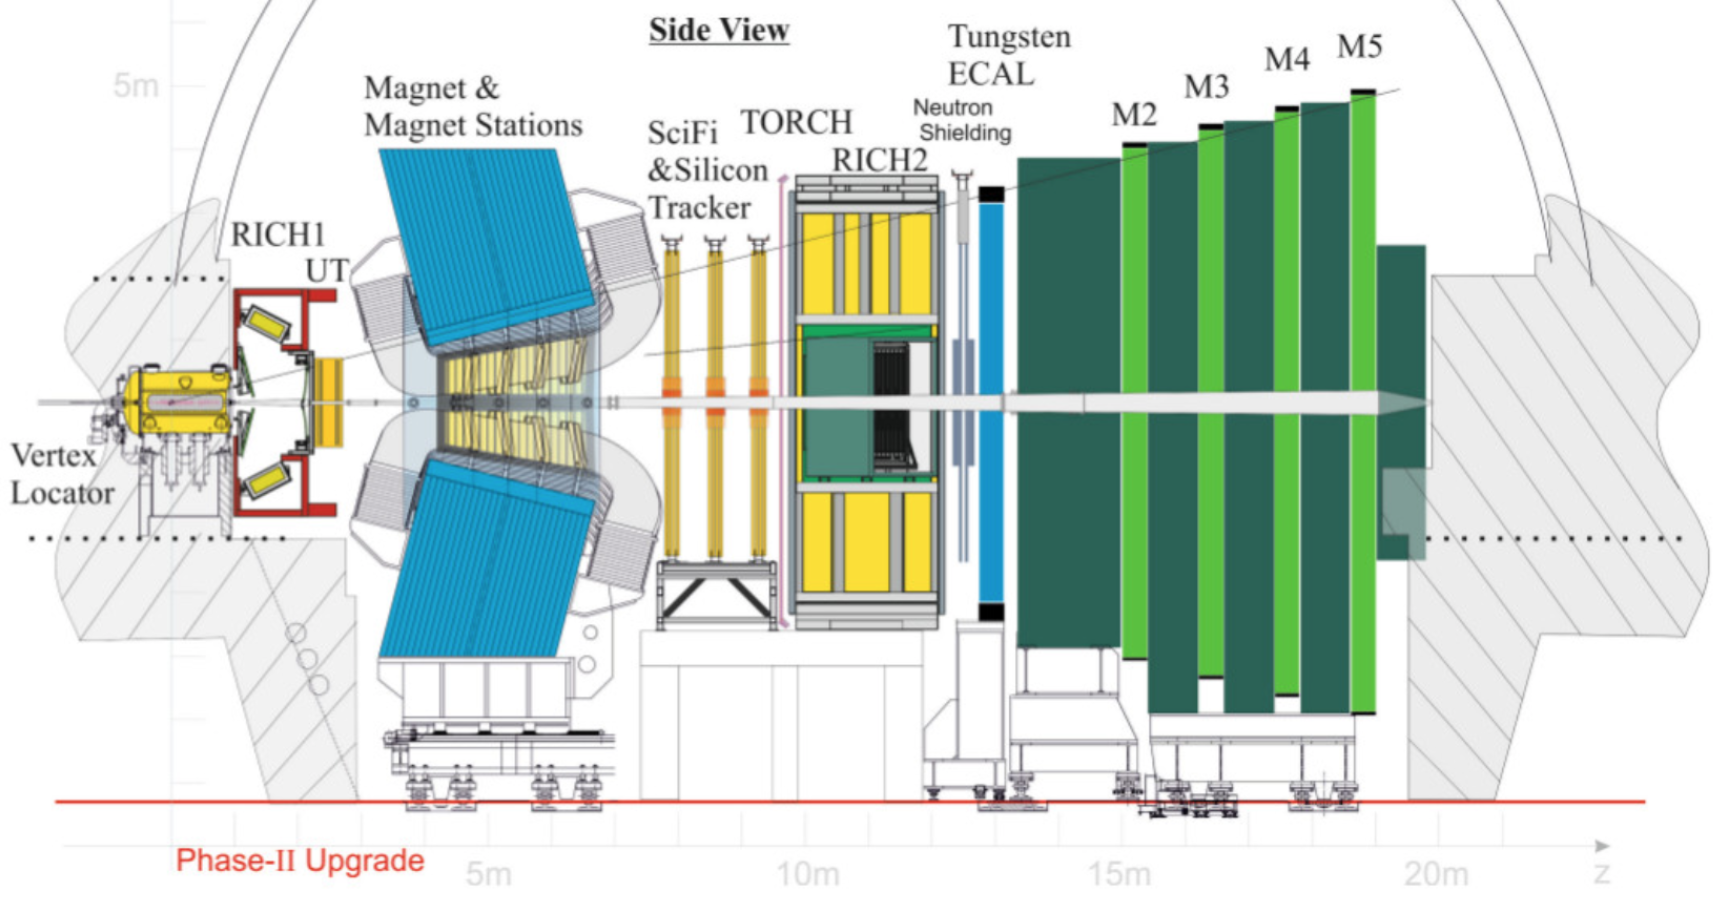
\includegraphics[width = 1.0\textwidth]{Figs/TORCH_location.png}
    \end{subfigure}%
    \begin{subfigure}{0.43\textwidth}
      \centering
      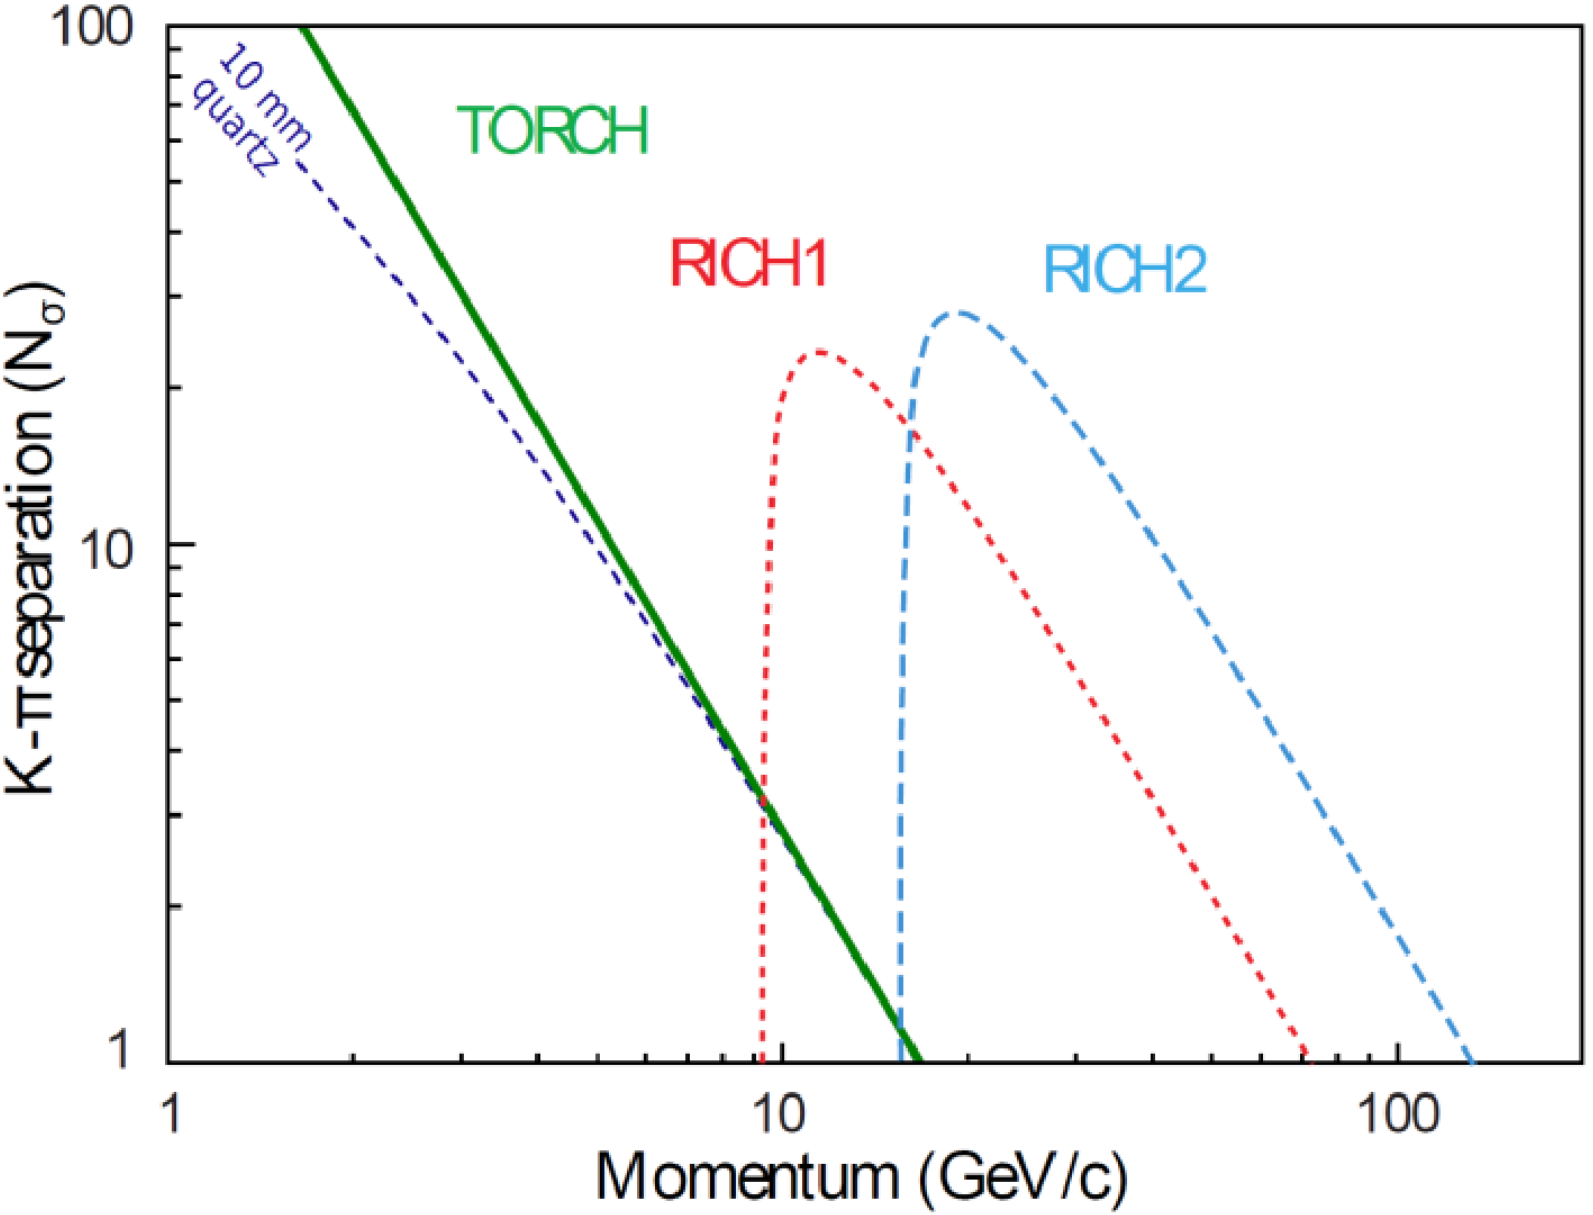
\includegraphics[width = 1.0\textwidth]{Figs/TORCH_RICH_separation.png}
    \end{subfigure}
  \end{figure}
\end{frame}

\begin{frame}{Introduction to TORCH}
  \vspace{0.0cm}
  \begin{center}
    {\large PID with Time-of-Flight, combined with Cherenkov information}
  \end{center}
  \begin{itemize}
    \item{Cover physics region inaccessible to RICH}
    \item{$\pi$-$K$ ToF difference over $\SI{10}{\meter}$ $\implies$ Aim for $10$-$\SI{15}{\pico\second}$ resolution}
    \item{Single-photon precision of $\SI{70}{\pico\second}$ with $\sim 30$ detected photons}
  \end{itemize}
  \begin{figure}
    \centering
    \begin{subfigure}{0.5\textwidth}
      \centering
      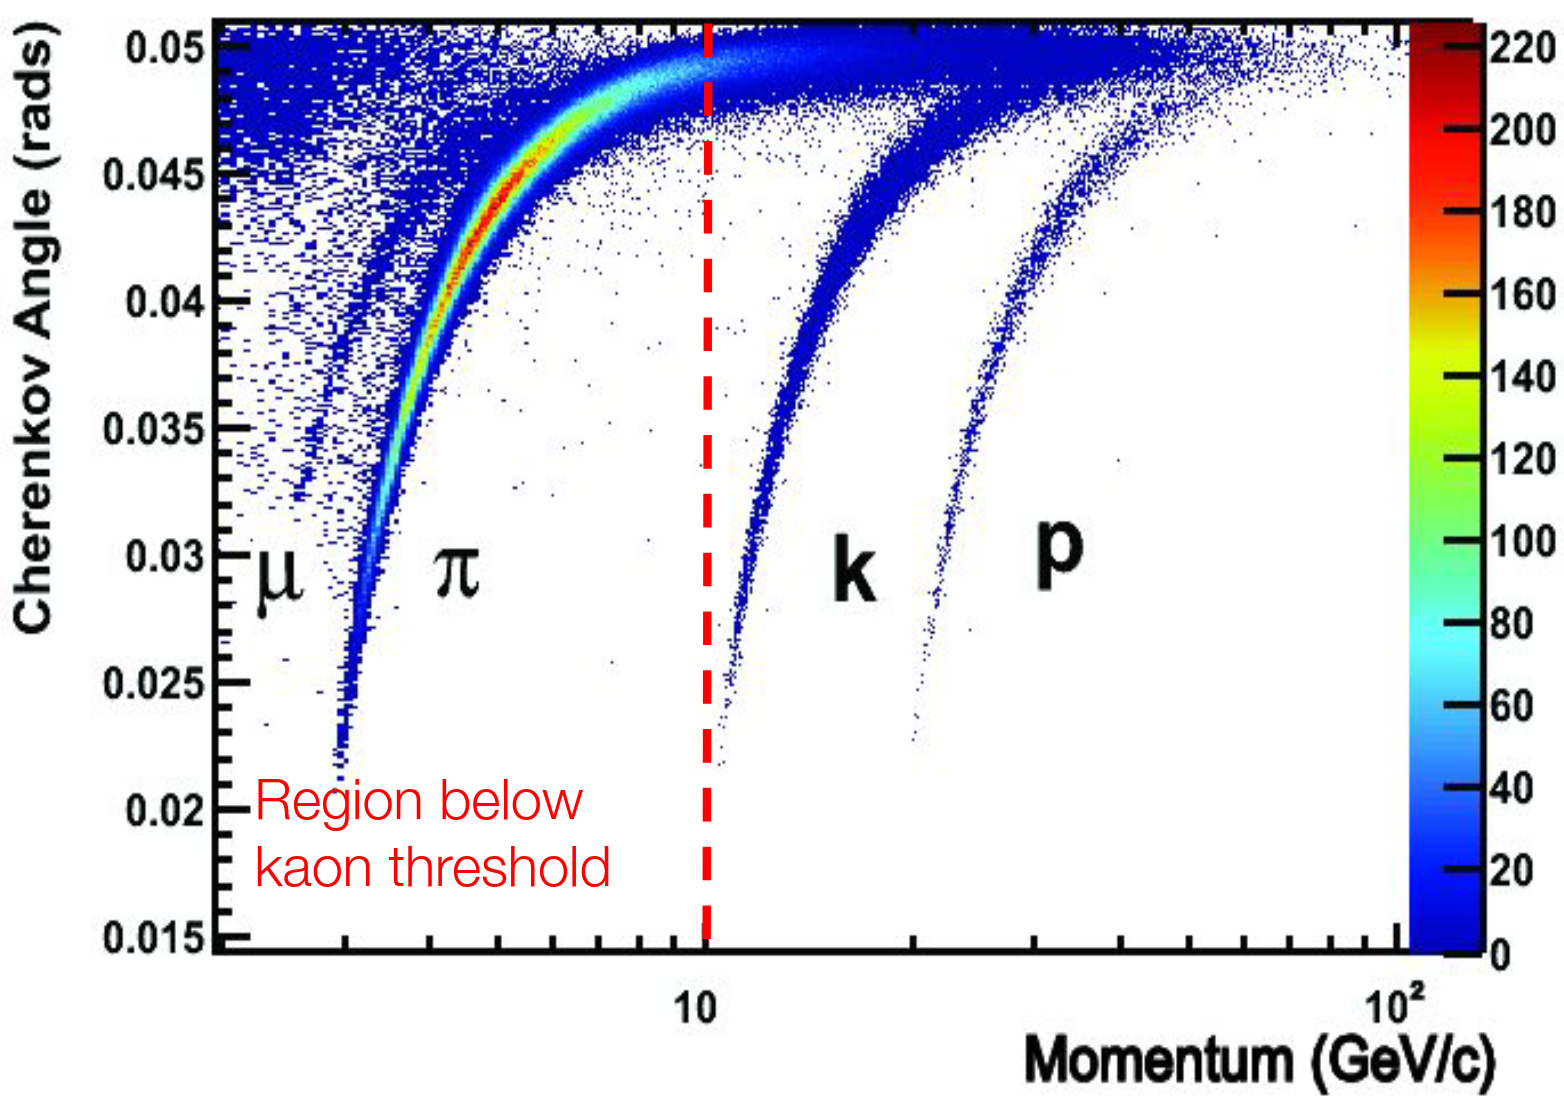
\includegraphics[width = 1.0\textwidth]{Figs/RICH_CherenkovAngle.png}
    \end{subfigure}%
    \begin{subfigure}{0.5\textwidth}
      \centering
      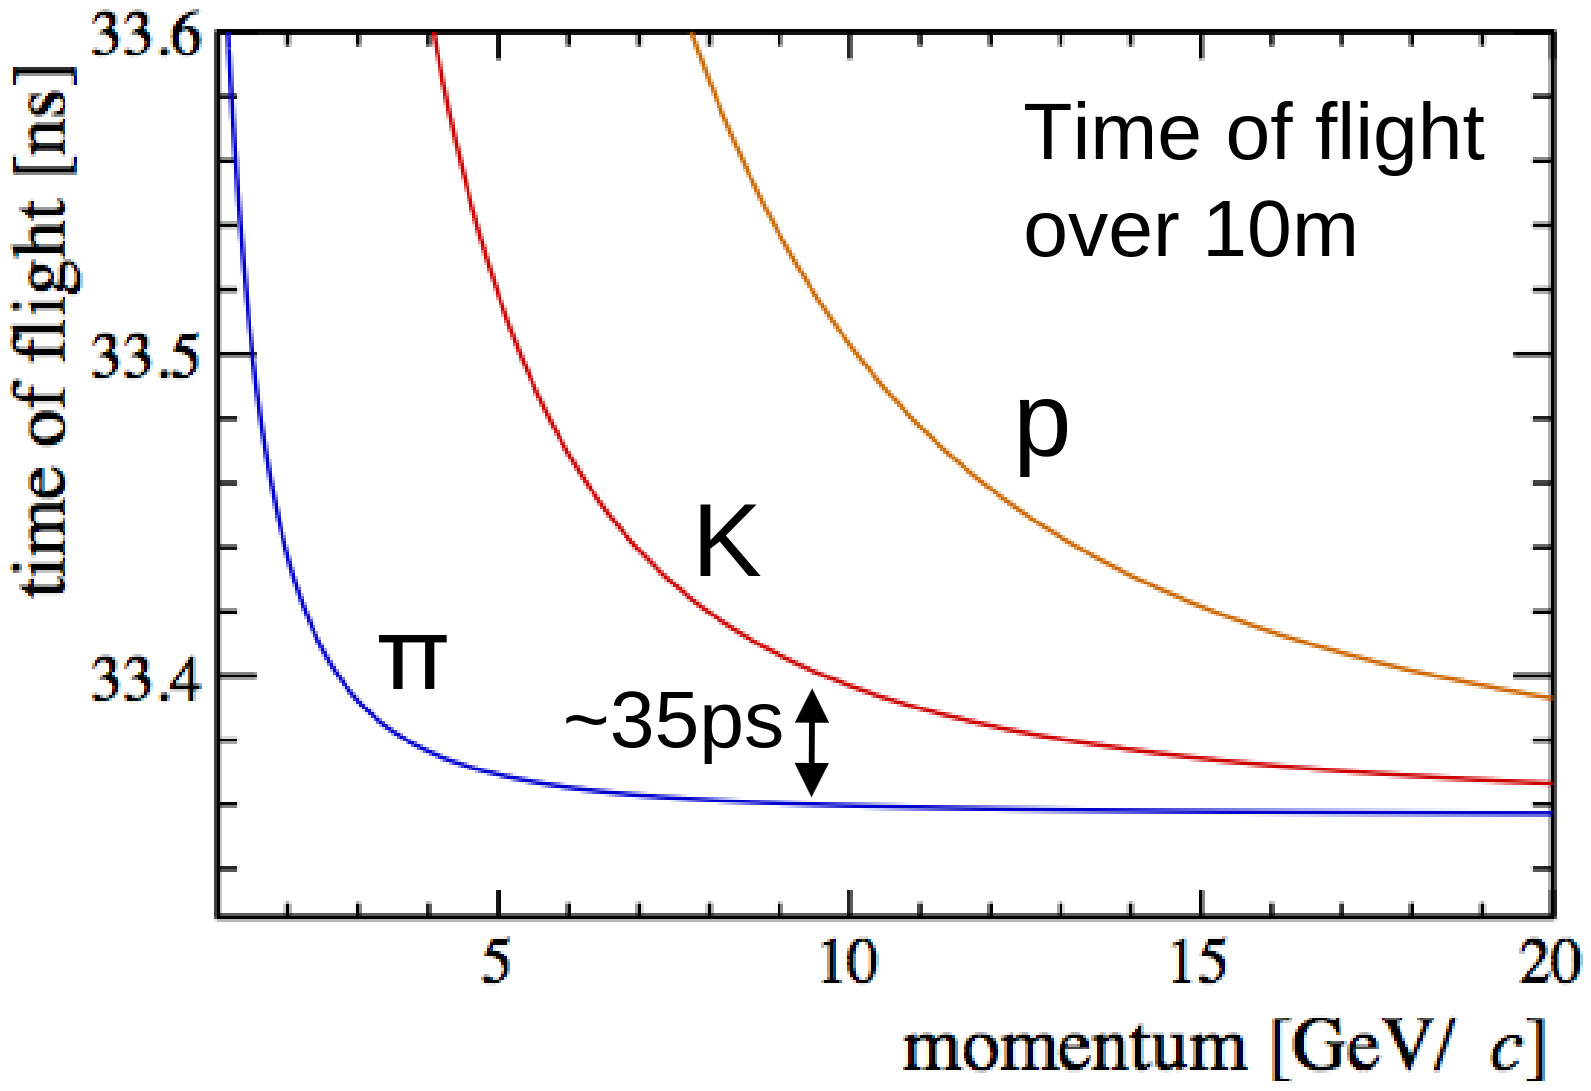
\includegraphics[width = 1.0\textwidth]{Figs/TORCH_ToF.png}
    \end{subfigure}
  \end{figure}
\end{frame}

\section{TORCH working principle}
\begin{frame}{TORCH working principle}
  \begin{columns}
    \begin{column}{0.60\textwidth}
      \begin{enumerate}
        \setlength\itemsep{1.0em}
        \item{Charged particle enters quartz}
        \item{Cherenkov photons promptly emitted}
        \item{Photons undergo internal reflection until they reach the top of the plate}
      \end{enumerate}
      \begin{figure}
        \centering
        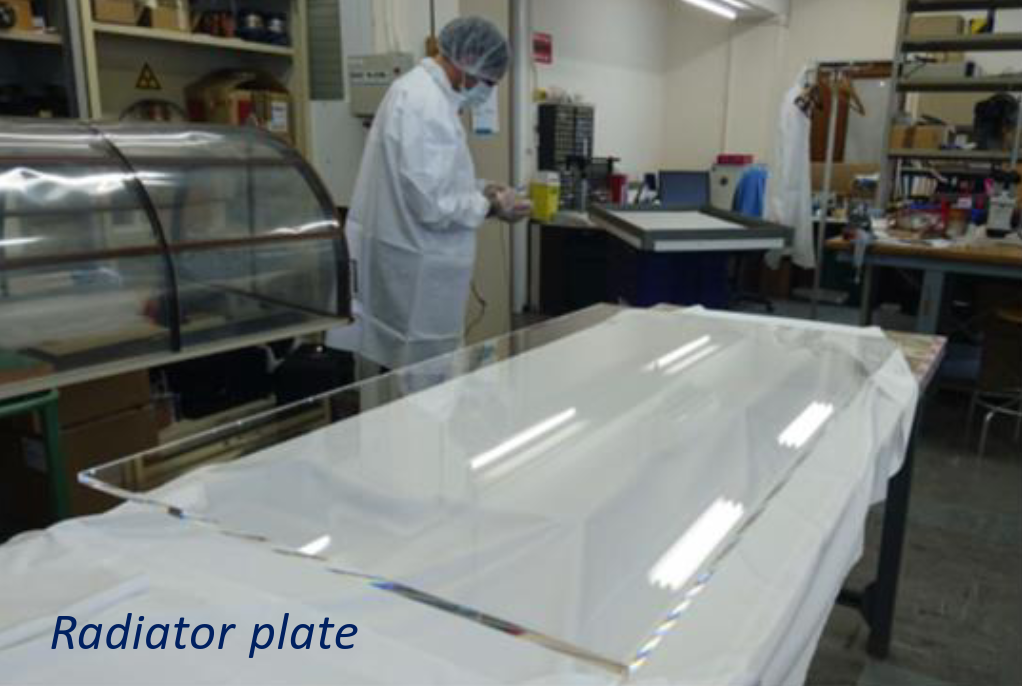
\includegraphics[width = 0.8\textwidth]{Figs/RadiatorPlate_lab.png}
      \end{figure}
    \end{column}
    \begin{column}{0.40\textwidth}
      \begin{figure}
        \centering
        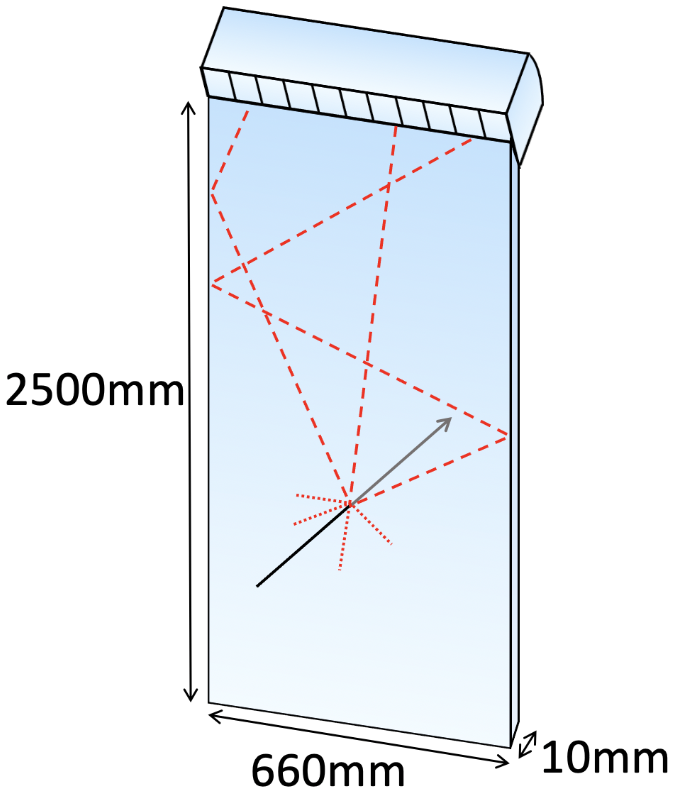
\includegraphics[width = 1.0\textwidth]{Figs/TORCH_FrontView.png}
      \end{figure}
    \end{column}
  \end{columns}
\end{frame}

\begin{frame}{TORCH working principle}
  \begin{columns}
    \begin{column}{0.65\textwidth}
      \begin{enumerate}
        \setlength\itemsep{1.0em}
        \item{Focus photons with cylindrical mirrror}
        \item{Image consists of hyperbolic ``bands''}
        \begin{itemize}
          \item{Compare with circular rings in RICH}
        \end{itemize}
        \item{Correct for chromatic dispersion using the Cherenkov angle obtained from $y'$}
      \end{enumerate}
      \begin{figure}
        \centering
        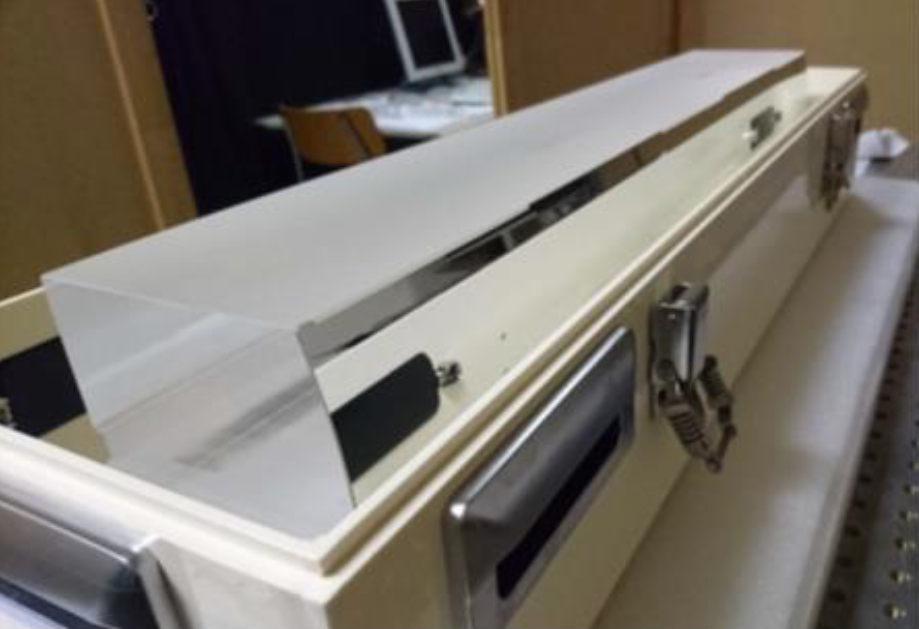
\includegraphics[width = 0.7\textwidth]{Figs/FocusingBlock_lab.png}
      \end{figure}
    \end{column}
    \begin{column}{0.35\textwidth}
      \begin{figure}
        \centering
        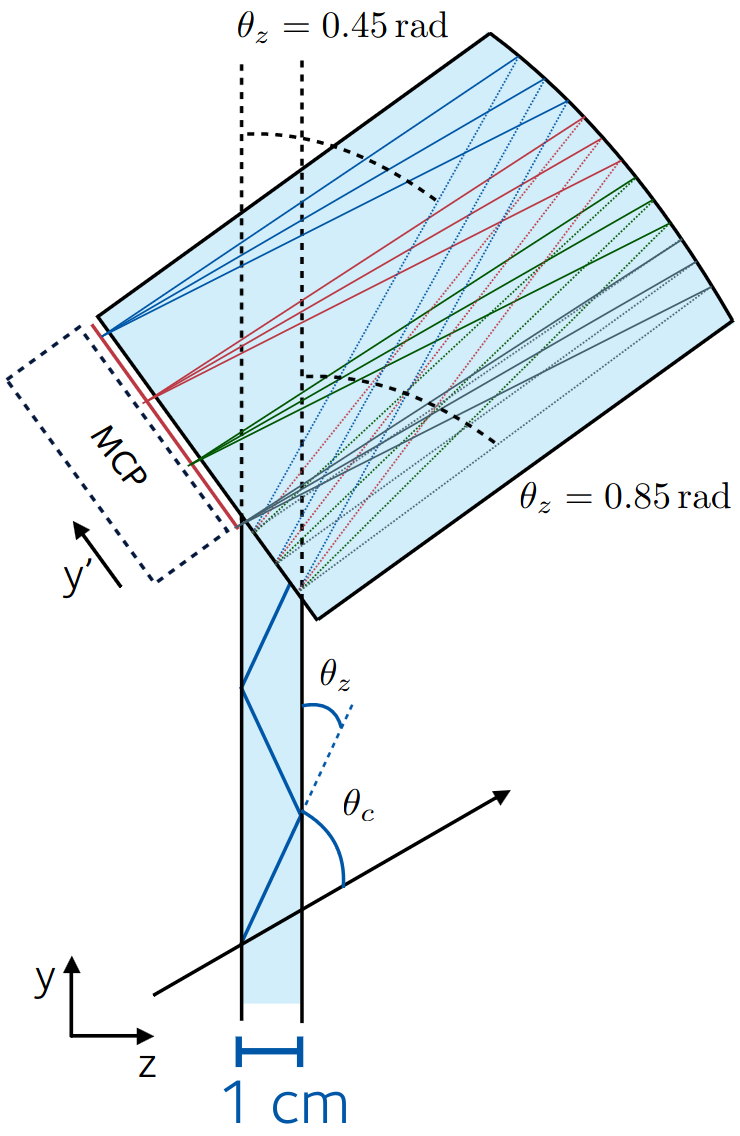
\includegraphics[width = 1.0\textwidth]{Figs/TORCH_SideView.png}
      \end{figure}
    \end{column}
  \end{columns}
\end{frame}

\section{Test beam analysis}
\begin{frame}{Test beam setup}
  \vspace{0.0cm}
  \begin{center}
    {\large Investigate TORCH performance with testbeam campaigns}
  \end{center}  
  \begin{itemize}
    \setlength\itemsep{0.3em}
    \item{Beam of pions and protons from the CERN T9 beamline}
    \item{Similar test beam area in 2018 and 2022 testbeams}
  \end{itemize}
  \begin{figure}
    \centering
    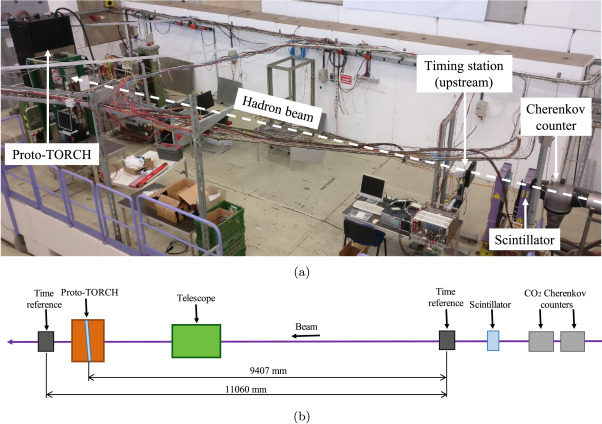
\includegraphics[width = 0.65\textwidth]{Figs/TORCH_testbeam_2018_setup.jpg}
  \end{figure}
\end{frame}

\begin{frame}{Reminder of Proto-TORCH}
  \begin{columns}
    \begin{column}{0.6\textwidth}
      \begin{itemize}
        \setlength\itemsep{1.0em}
        \item{Prototype of TORCH}
        \item{Full width, half height}
        \item{Nikon glass with polished surfaces}
      \end{itemize}
      \begin{figure}
        \centering
        \begin{overpic}[percent,width=0.7\textwidth,trim={0 7.5cm 0 0},clip=true]{Figs/TORCH_testbeam_2018_structure.jpg}
          \put(10,-10){\vector(1.0,1.5){20}}
          \put(-5,-20){Half height quartz radiator plate}
        \end{overpic}
      \end{figure}
    \end{column}
    \begin{column}{0.4\textwidth}
      \begin{figure}
        \centering
        \begin{overpic}[percent,width=0.9\textwidth,trim={4.5cm 0.5cm 0 5cm},clip=true]{Figs/TORCH_testbeam_2018_structure.jpg}
          \put(-10,100){\vector(1.0,-0.5){30}}
          \put(-50,100){Focusing block}
          \put(30,102){\vector(0.3,-1.0){10}}
          \put(10,105){MCPs and electronics}
        \end{overpic}
      \end{figure}
    \end{column}
  \end{columns}
\end{frame}

\begin{frame}{Reminder of Photek MCP-PMT}
  \begin{itemize}
    \setlength\itemsep{0.7em}
    \item{Photon detector: MicroChannel Plate PhotoMultiplier Tube}
    \begin{itemize}
      \item[-]{T.M. Conneely \textit{et al} 2016 \textit{JINST} \textbf{10} C05003}
    \end{itemize}
    \item{$53\times 53\si{\milli\meter\squared}$ active area}
    \item{$8$ columns, each with $64$ pixels}
    \item{Effectively $128$ pixels with charge sharing}
  \end{itemize}
  \begin{figure}
    \centering
    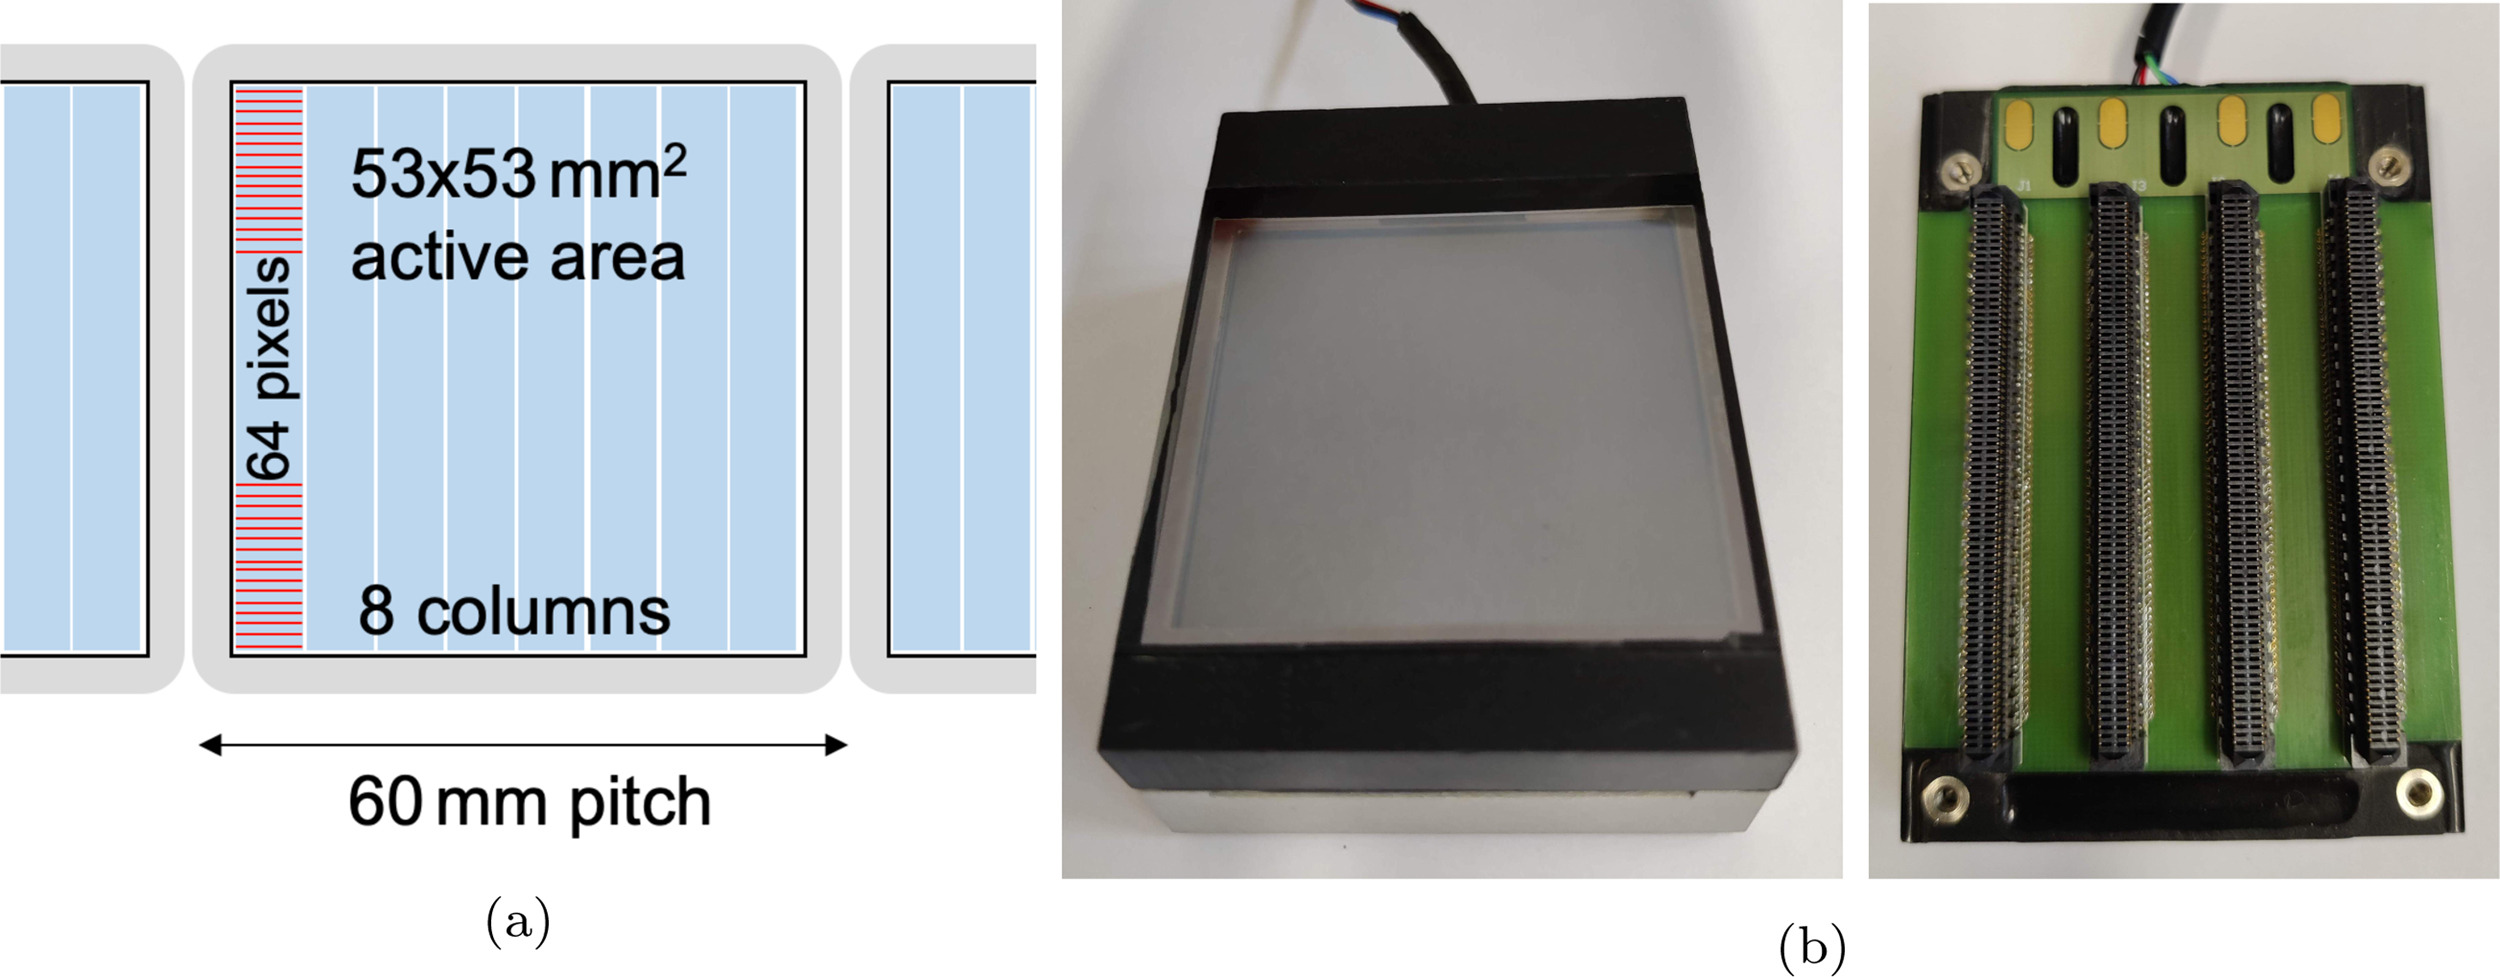
\includegraphics[width = 1.0\textwidth,trim={0 0.5cm 0 0},clip=true]{Figs/TORCH_testbeam_2018_MCPPMT.jpg}
  \end{figure}
\end{frame}

\begin{frame}{Reminder of 2018 test beam analysis}
  \vspace{0.0cm}
  \begin{center}
    {\large 2018 test beam analysis paper recently published:\\}
    {\small \href{https://www.sciencedirect.com/science/article/pii/S0168900223001717}{Nucl. Instrum. Methods \textbf{A1050} (2023)}}
  \end{center}
  \begin{itemize}
    \setlength\itemsep{1.0em}
    \item{Single-photon time resolution down to $\SI{70}{\pico\second}$ achieved}
    \item{Degraded resolution for tracks entering at the bottom, as expected}
    \begin{itemize}
      \item{Uncertainty in chromatic dispersion scales with photon path length}
      \item{Improvements expected with further electronics calibrations}
    \end{itemize}
  \end{itemize}
  \begin{figure}
    \centering
    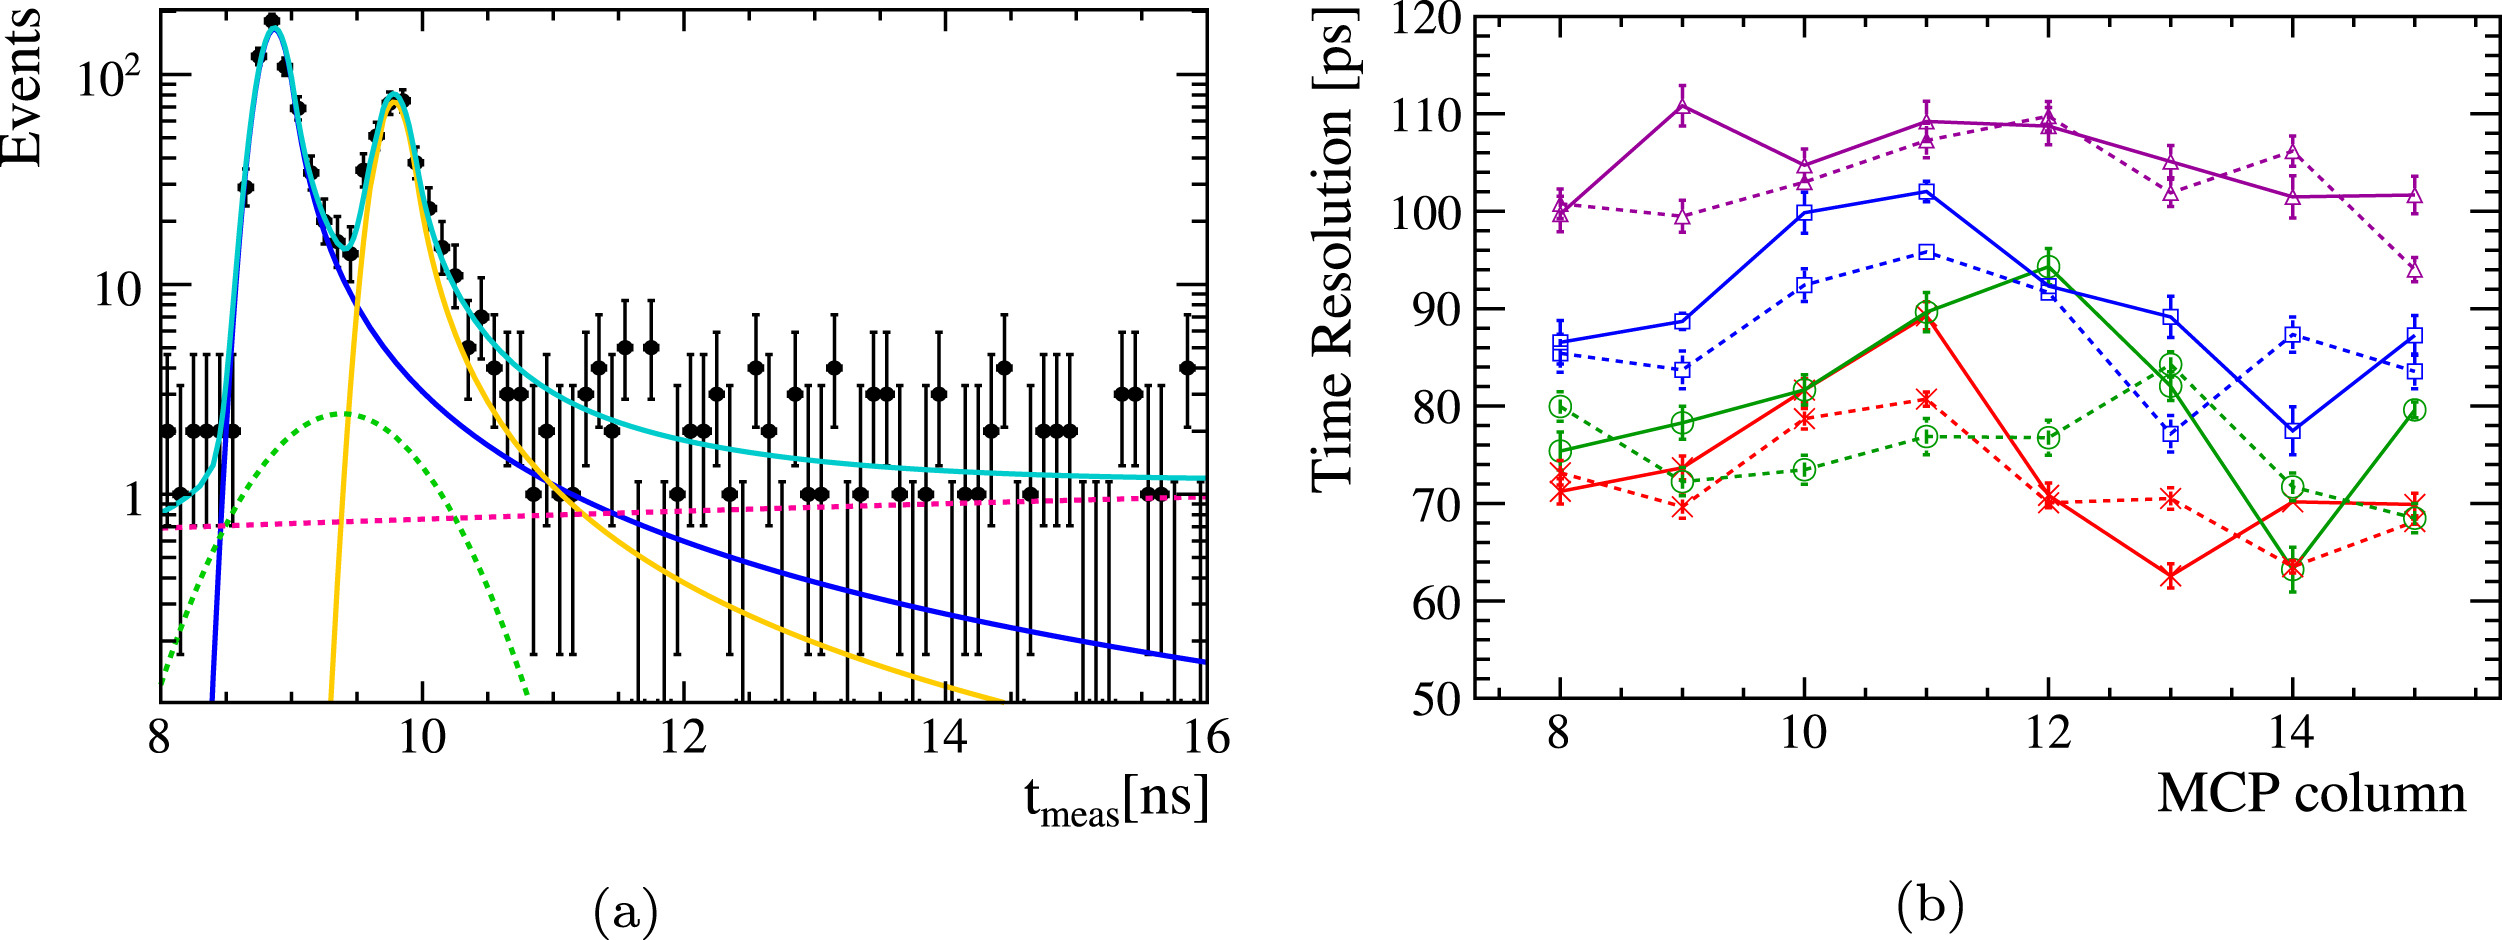
\includegraphics[width = 1.0\textwidth]{Figs/TORCH_testbeam_2018_TimeResolution.jpg}
  \end{figure}
\end{frame}

\section{2022 test beam analysis}
\begin{frame}{2022 test beam analysis}
  \vspace{0.0cm}
  \begin{center}
    {\large Back to T9, with several new goals:}
  \end{center}
  \begin{enumerate}
    \setlength\itemsep{1.0em}
    \item{Additional, fully instrumented, MCP-PMT tubes (7 in total)}
    \item{Wide range of beam momenta ($3$, $5$, $8$, $\SI{10}{\giga\eV/c}$ and higher)}
    \item{Aim to achieve a first demonstration of PID separation in TORCH}
  \end{enumerate}
  \begin{figure}
    \centering
    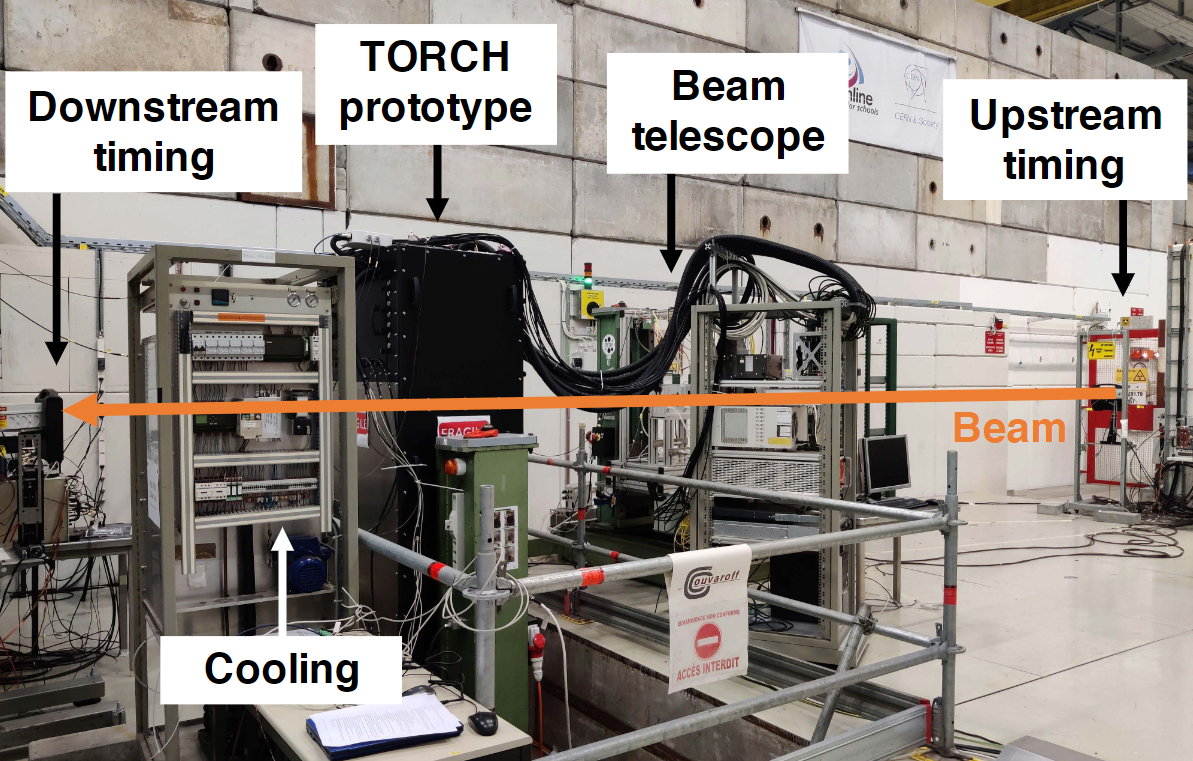
\includegraphics[width = 0.6\textwidth]{Figs/TORCH_overview.png}
  \end{figure}
\end{frame}

\begin{frame}{2022 test beam analysis}
  \vspace{0.0cm}
  \begin{center}
    {\large Global hit map looks as expected}
  \end{center}
  \begin{enumerate}
    \setlength\itemsep{0.5em}
    \item{Hit pattern seen across 6 MCP-PMT tubes}
    \begin{itemize}
      \item{Original MCP B is fully efficient, while MCP A shows some degradation}
    \end{itemize}
    \item{Hit pattern shows some inefficient MCPs and miscalibrated electronics}
    \item{Proper time reference channel present in (almost) all columns}
  \end{enumerate}
  \vspace{0.01cm}
  \begin{figure}
    \centering
    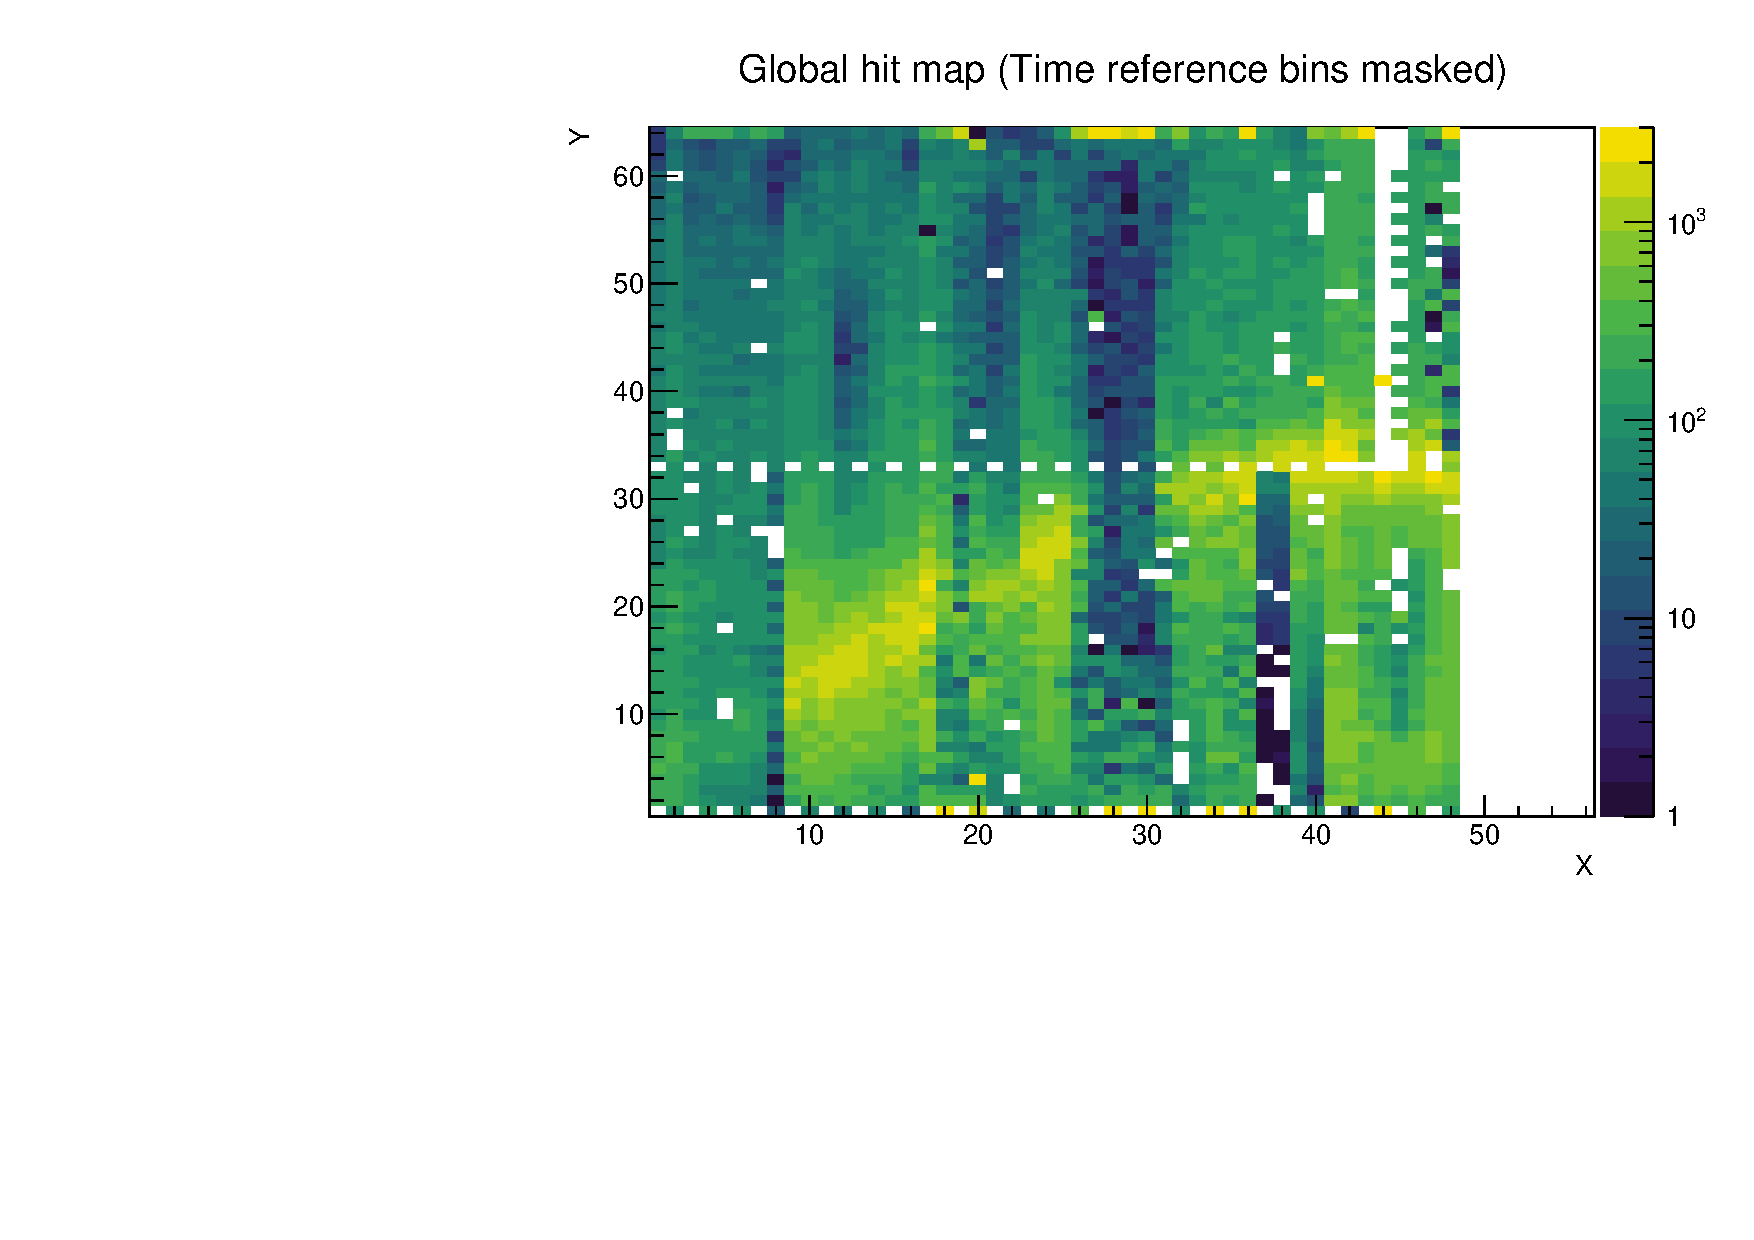
\includegraphics[width = 0.6\textwidth]{Figs/GlobalHitMap_Run480.pdf}
  \end{figure}
\end{frame}

\begin{frame}{2022 test beam analysis}
  \vspace{0.0cm}
  \begin{center}
    {\large Focus on MCP A and B for now}
  \end{center}
  \vspace{0.1cm}
  \begin{enumerate}
    \setlength\itemsep{0.0em}
    \item{Some non-uniformity in QE and gain seen in MCP C, D and F}
    \item{Electronics and new MCPs need to be understood better}
    \begin{itemize}
      \item{Improve stability and reliability}
      \item{NINO thresholds need to be optimised}
      \item{Boards C-F are under calibration using a test system at Bristol}
    \end{itemize}
  \end{enumerate}
  \vspace{-0.04cm}
  \begin{figure}
    \centering
    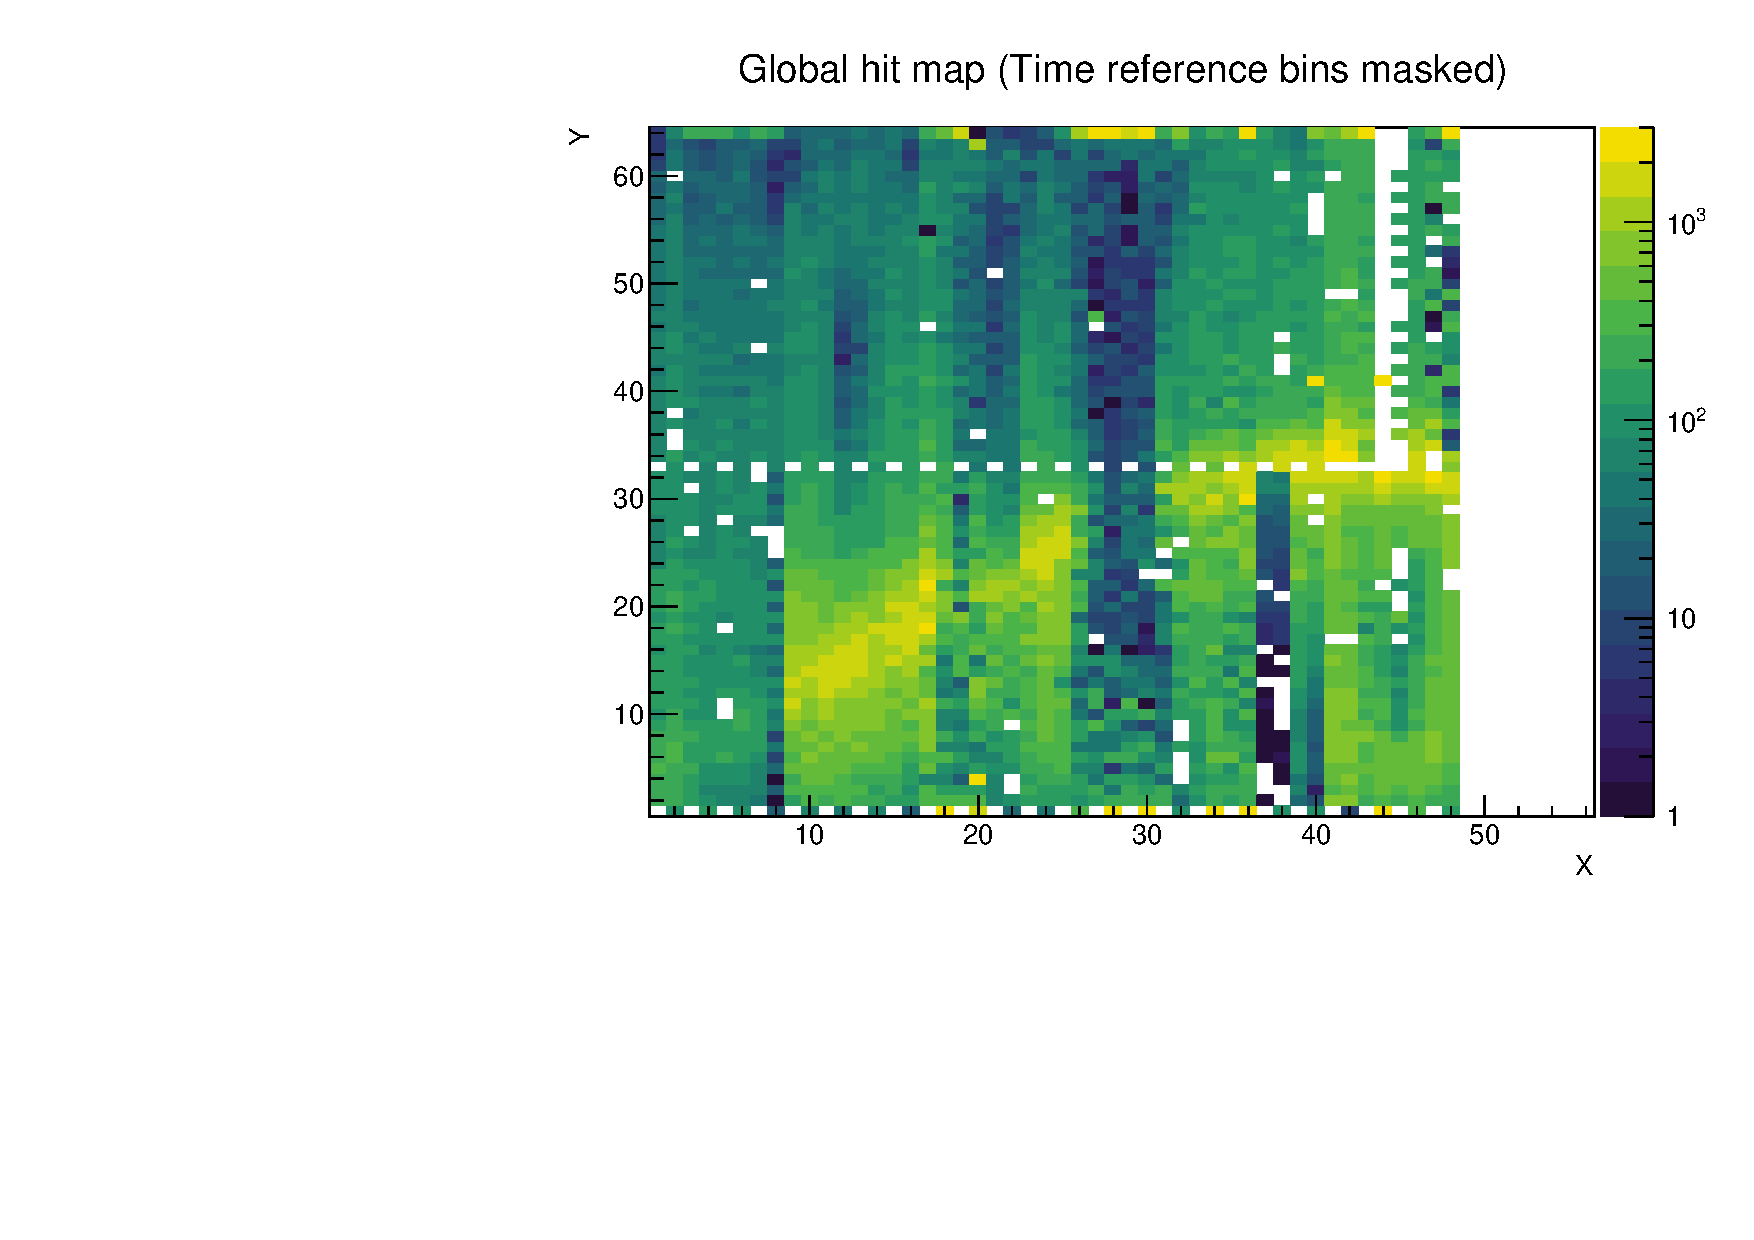
\includegraphics[width = 0.6\textwidth]{Figs/GlobalHitMap_Run480.pdf}
  \end{figure}
\end{frame}

\begin{frame}{2022 test beam analysis}
  \begin{columns}
    \begin{column}{0.7\textwidth}
      \begin{itemize}
        \setlength\itemsep{1.0em}
        \item{Study positions 1, 8, 9, 10, 11, 12}
        \item{Below: Comparison of position 1 between 2018 and 2022 data $\implies$ Perfect agreement!}
      \end{itemize}
      \vspace{-0.3cm}
      \begin{figure}
        \centering
        \caption*{2018\qquad\qquad\qquad\qquad\qquad\qquad 2022}
        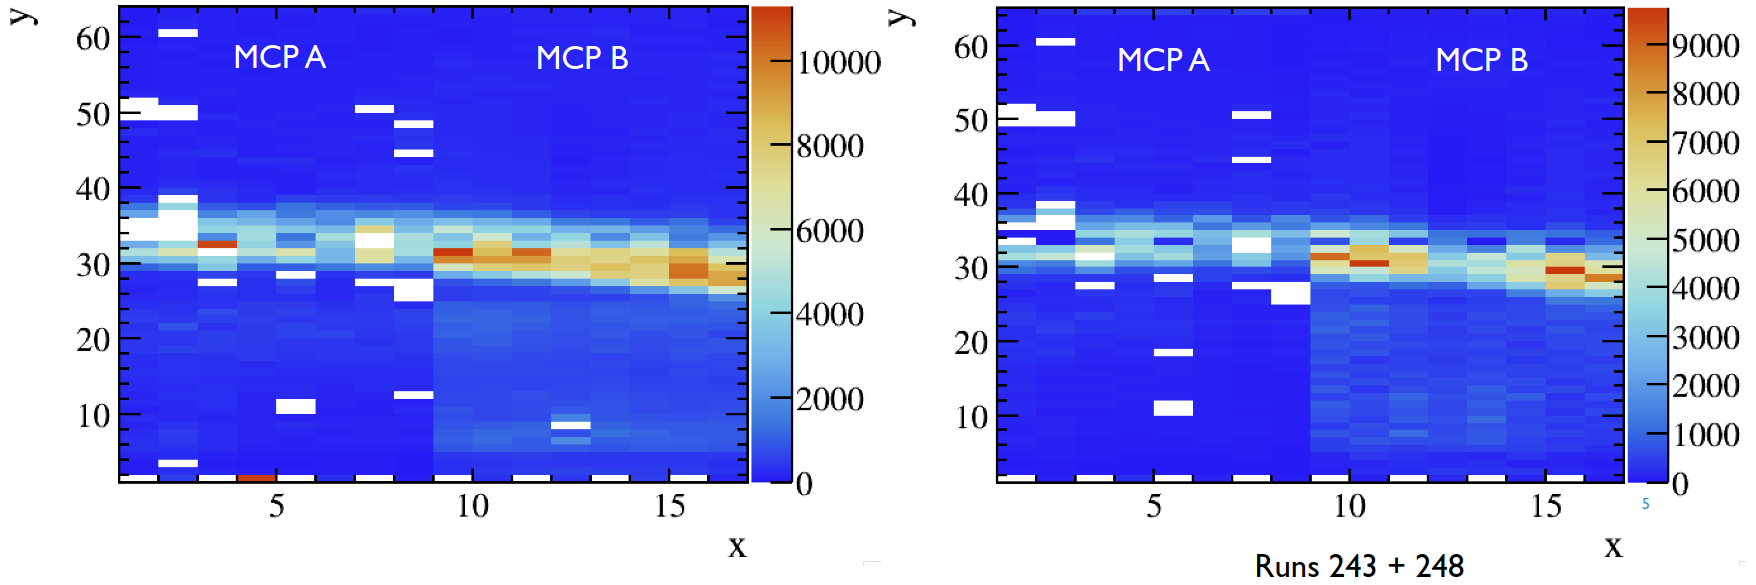
\includegraphics[width = 1.0\textwidth]{Figs/TORCH_testbeam_2018_2022_comparison.png}
      \end{figure}
      \begin{itemize}
        \item{This talk: Preliminary results from position 8}
        \begin{itemize}
          \item{Never studied before!}
        \end{itemize}
      \end{itemize}
    \end{column}
    \begin{column}{0.3\textwidth}
      \begin{figure}
        \centering
        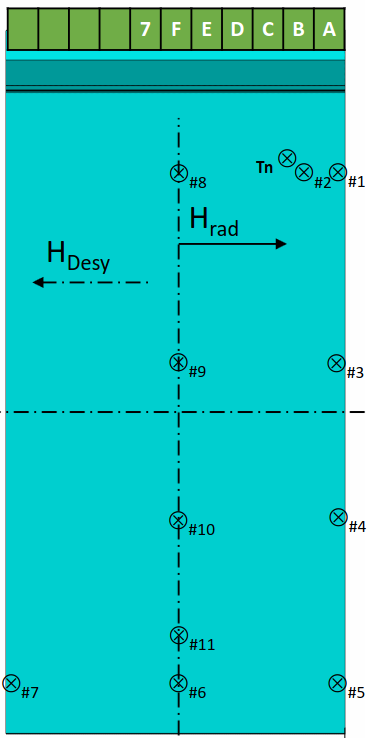
\includegraphics[width = 0.9\textwidth]{Figs/BeamPositions.png}
      \end{figure}
    \end{column}
  \end{columns}
\end{frame}

\begin{frame}{2022 test beam analysis}
  \vspace{0.0cm}
  \begin{center}
    {\large Check time of flight between external time references}\\
    {\normalsize Expected time difference at $\SI{3}{\giga\eV/c}$: $\SI{1.6}{\nano\second}$}
  \end{center}
  \begin{figure}
    \centering
    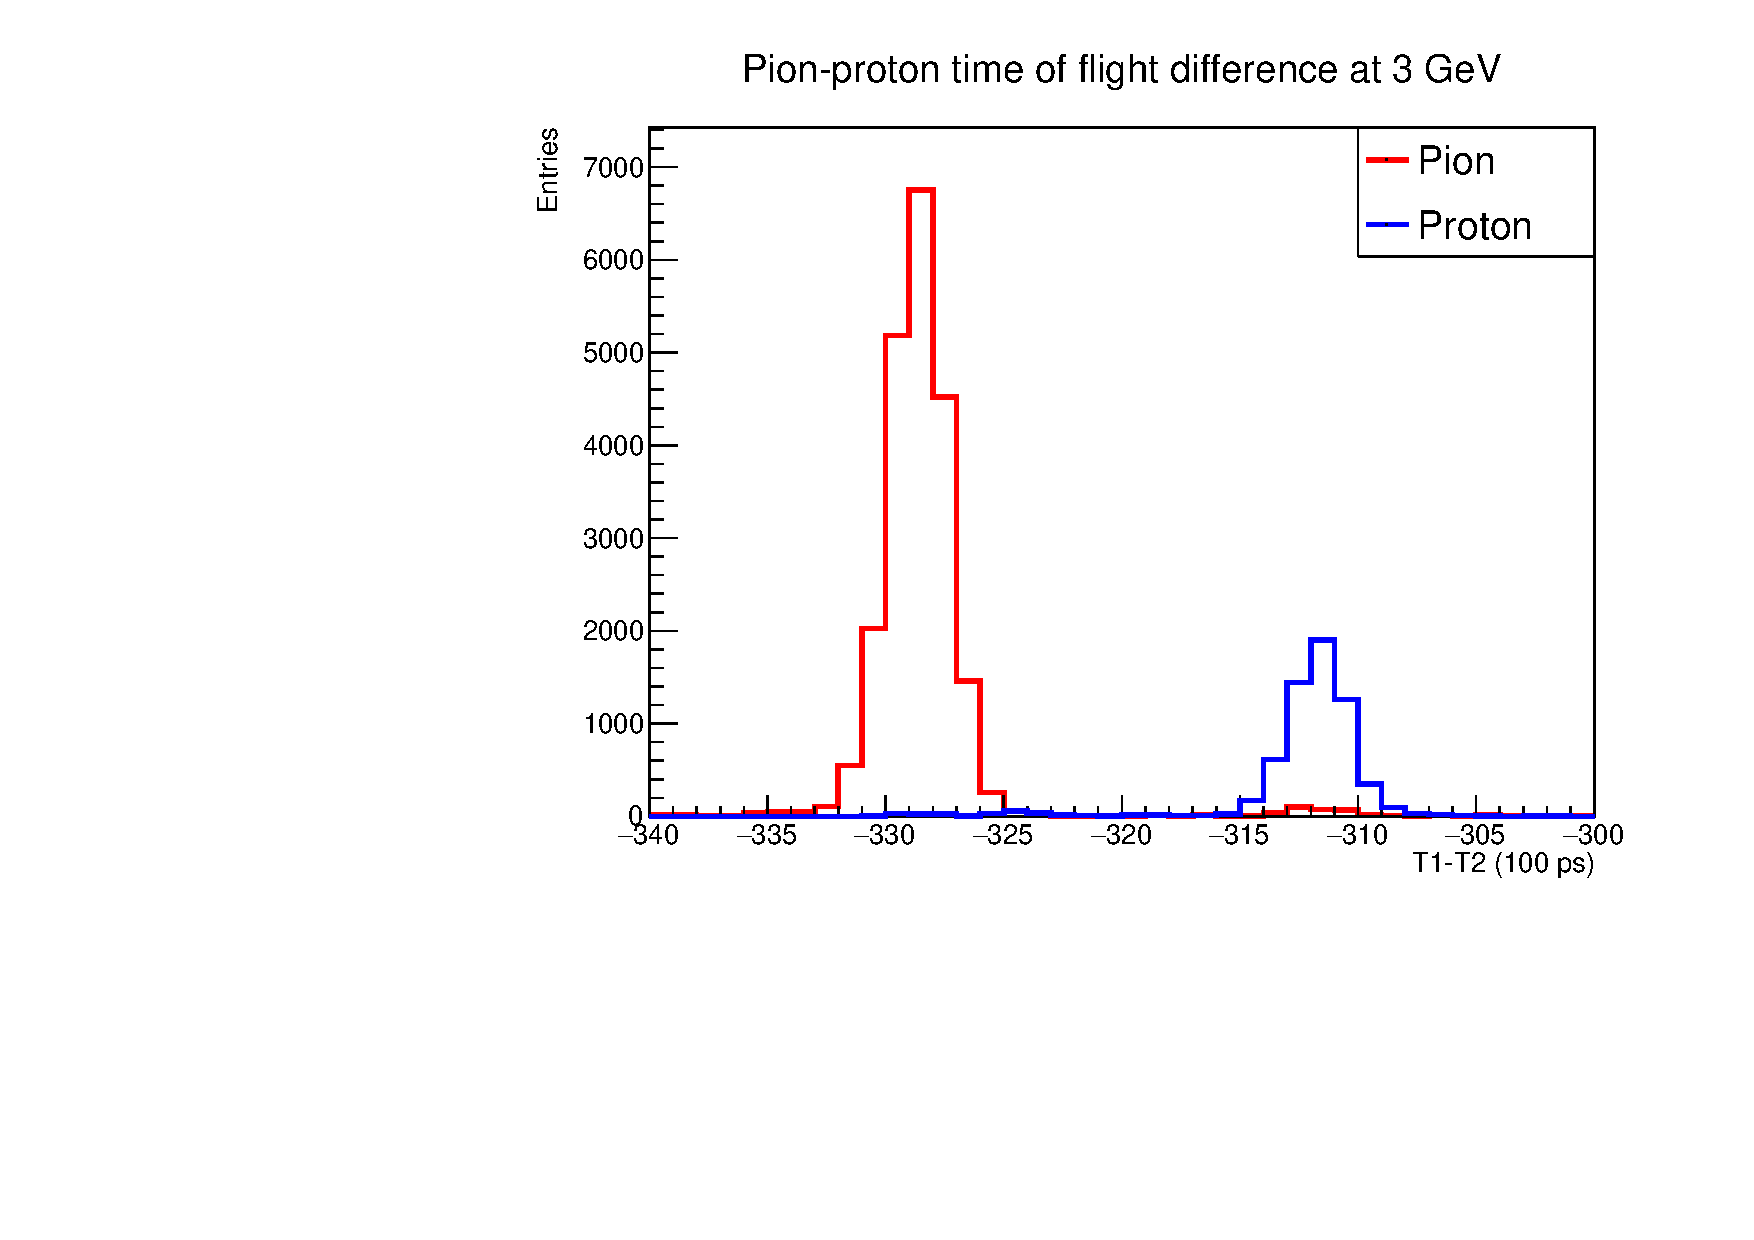
\includegraphics[width = 0.7\textwidth]{Figs/PionProton_TimeDiff_3GeV.pdf}
  \end{figure}
\end{frame}

\begin{frame}{2022 test beam analysis}
  \vspace{0.0cm}
  \begin{center}
    {\large Check time of flight between external time references}\\
    {\normalsize Expected time difference at $\SI{5}{\giga\eV/c}$: $\SI{0.59}{\nano\second}$}
  \end{center}
  \begin{figure}
    \centering
    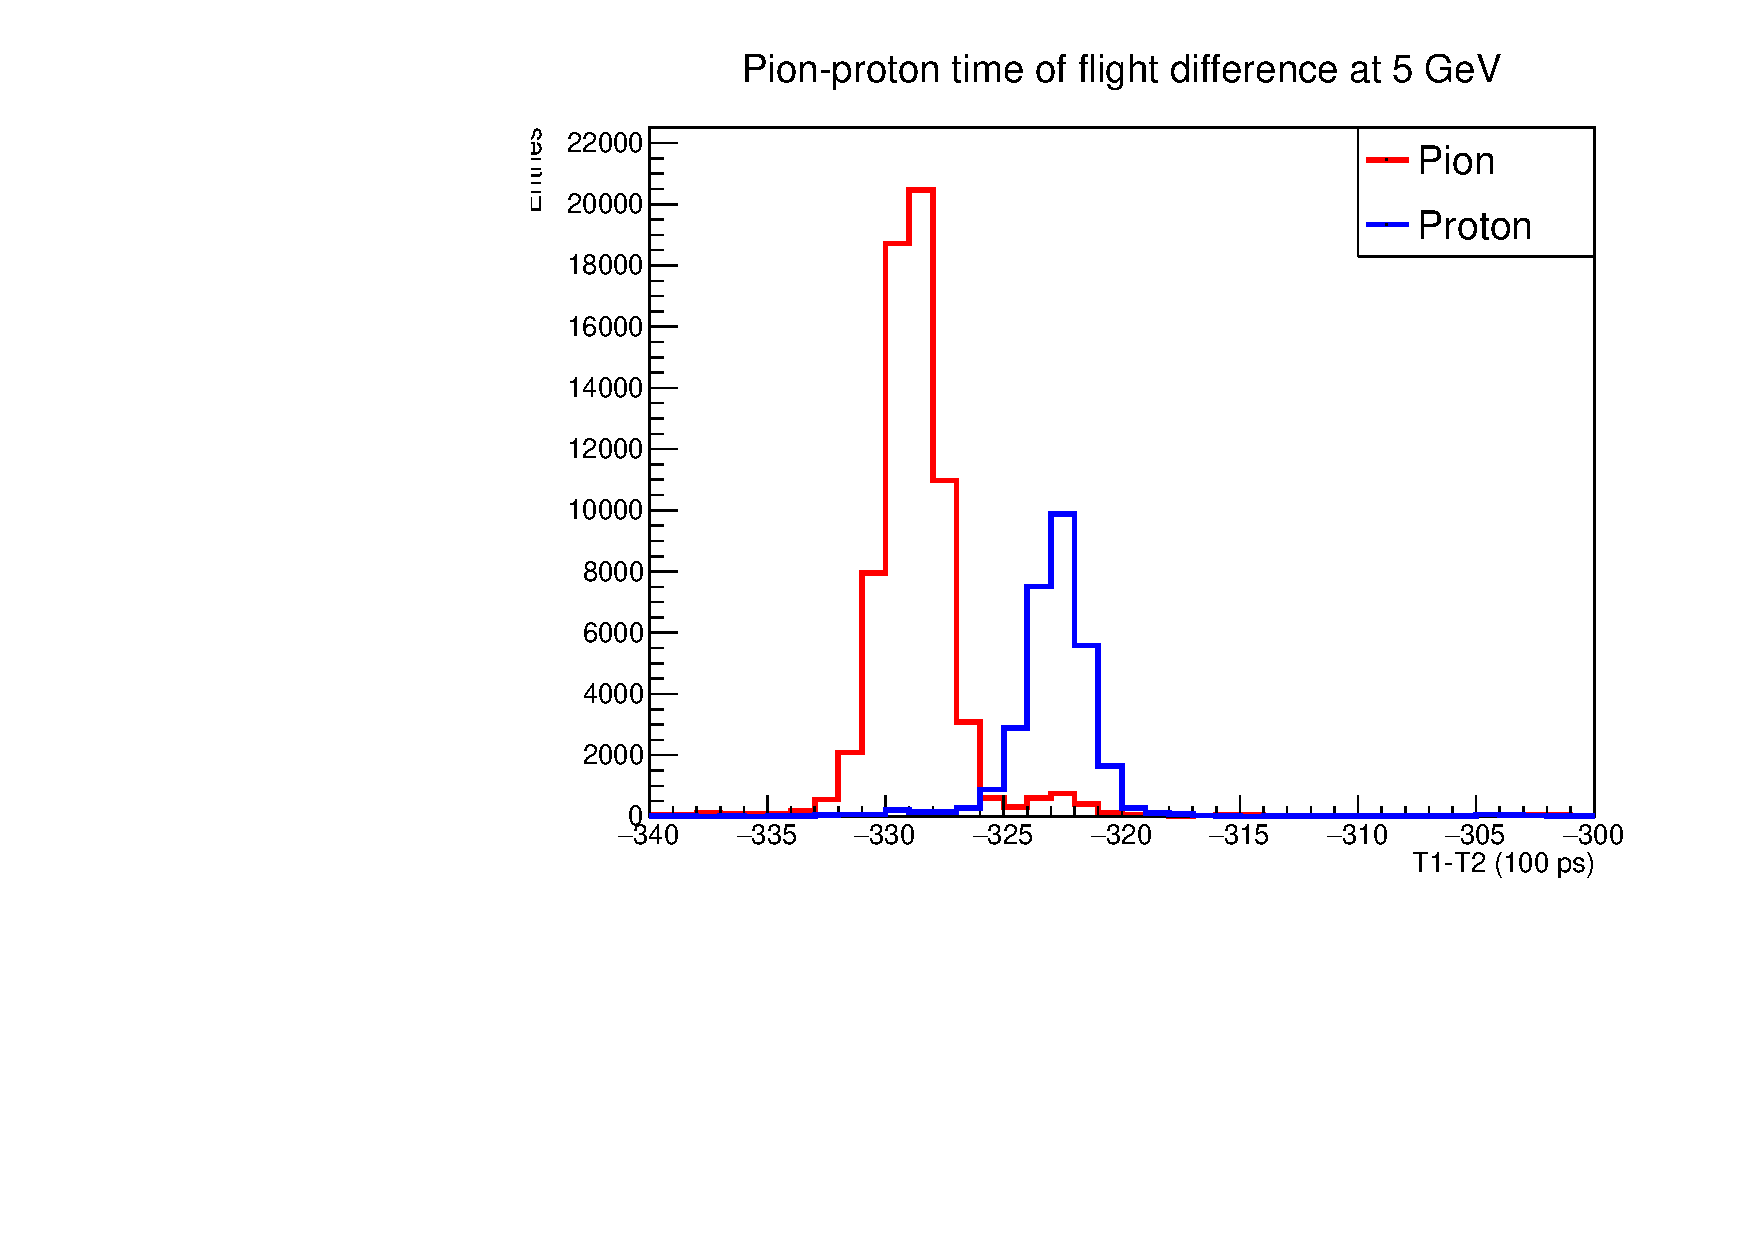
\includegraphics[width = 0.7\textwidth]{Figs/PionProton_TimeDiff_5GeV.pdf}
  \end{figure}
\end{frame}

\begin{frame}{2022 test beam analysis}
  \vspace{0.0cm}
  \begin{center}
    {\large Check time of flight between external time references}\\
    {\normalsize Expected time difference at $\SI{8}{\giga\eV/c}$: $\SI{0.23}{\nano\second}$}
  \end{center}
  \begin{figure}
    \centering
    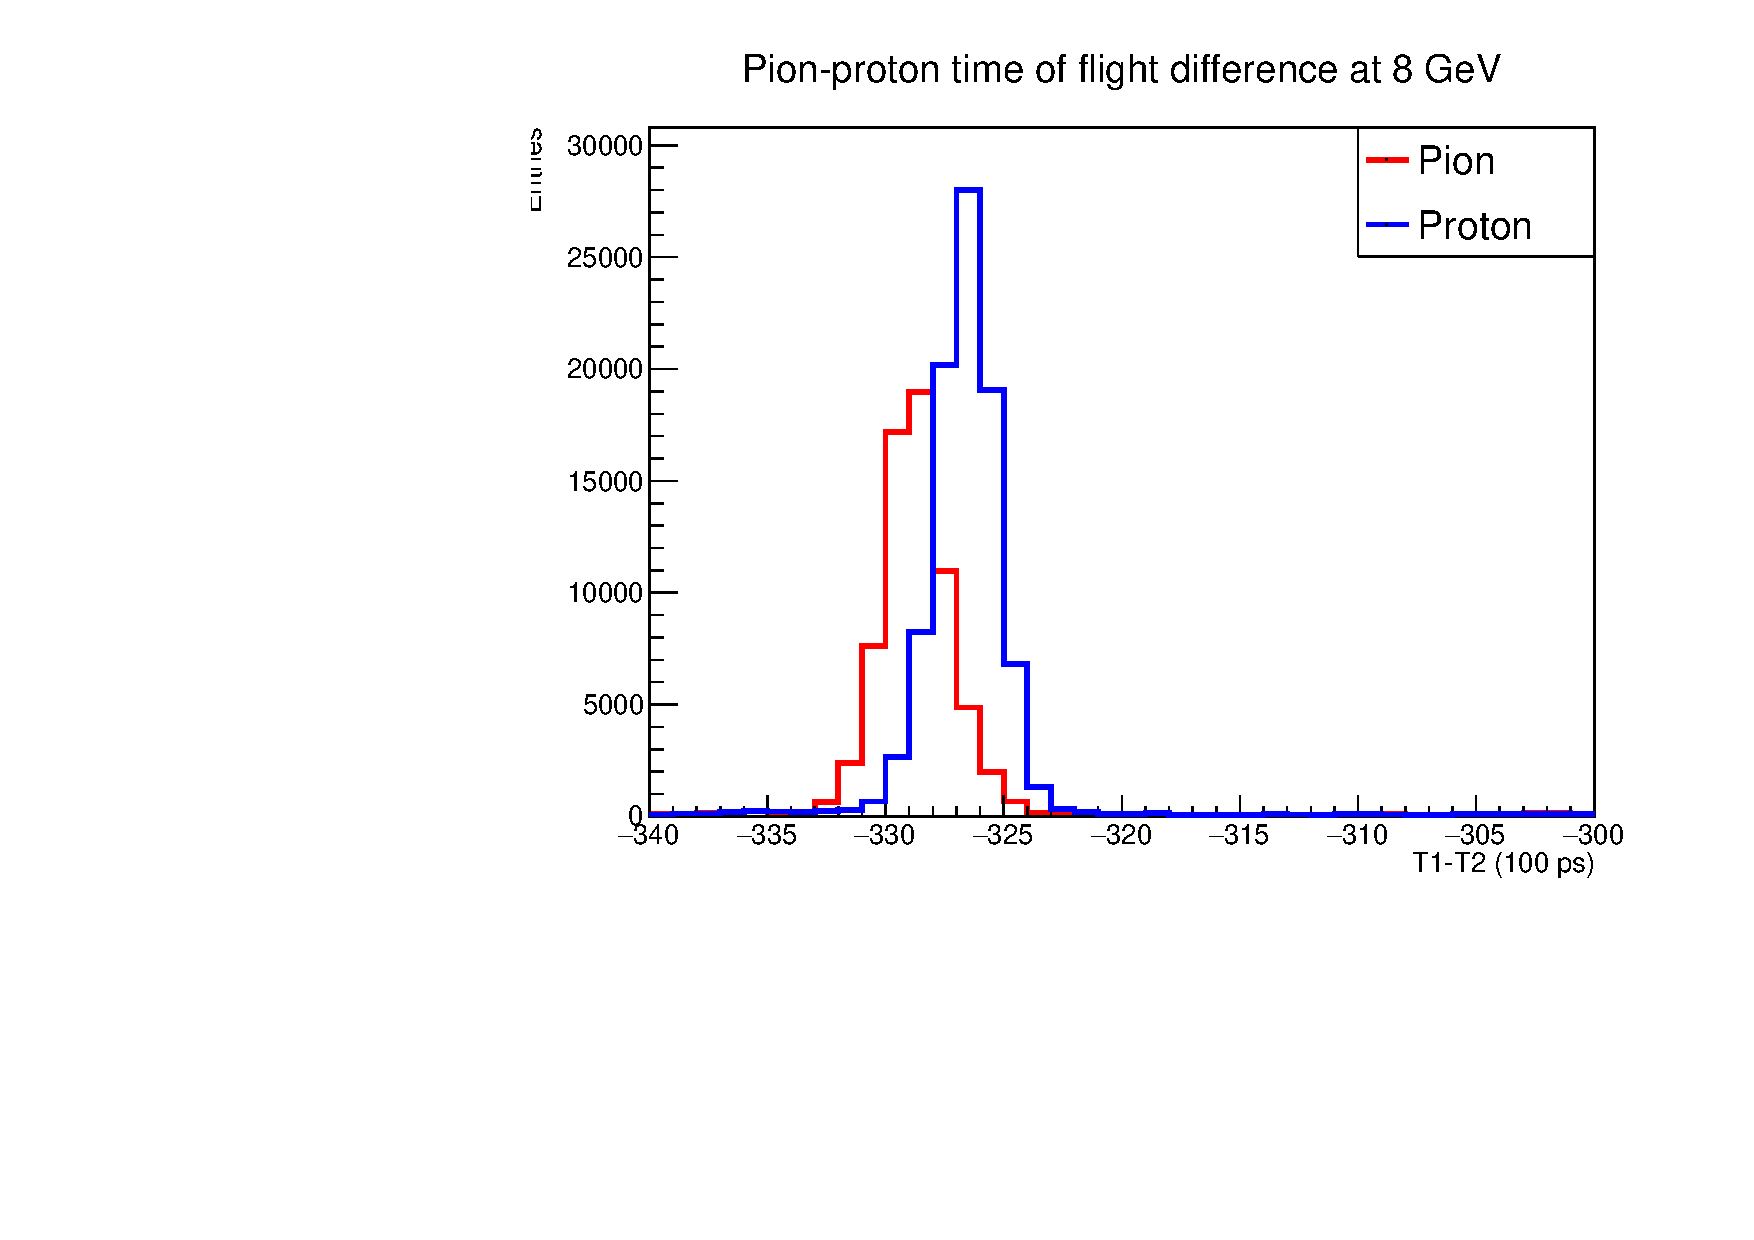
\includegraphics[width = 0.7\textwidth]{Figs/PionProton_TimeDiff_8GeV.pdf}
  \end{figure}
\end{frame}

\begin{frame}{2022 test beam analysis}
  \vspace{0.0cm}
  \begin{center}
    {\large Check time of flight between external time references}\\
    {\normalsize Expected time difference at $\SI{10}{\giga\eV/c}$: $\SI{0.15}{\nano\second}$}
  \end{center}
  \begin{figure}
    \centering
    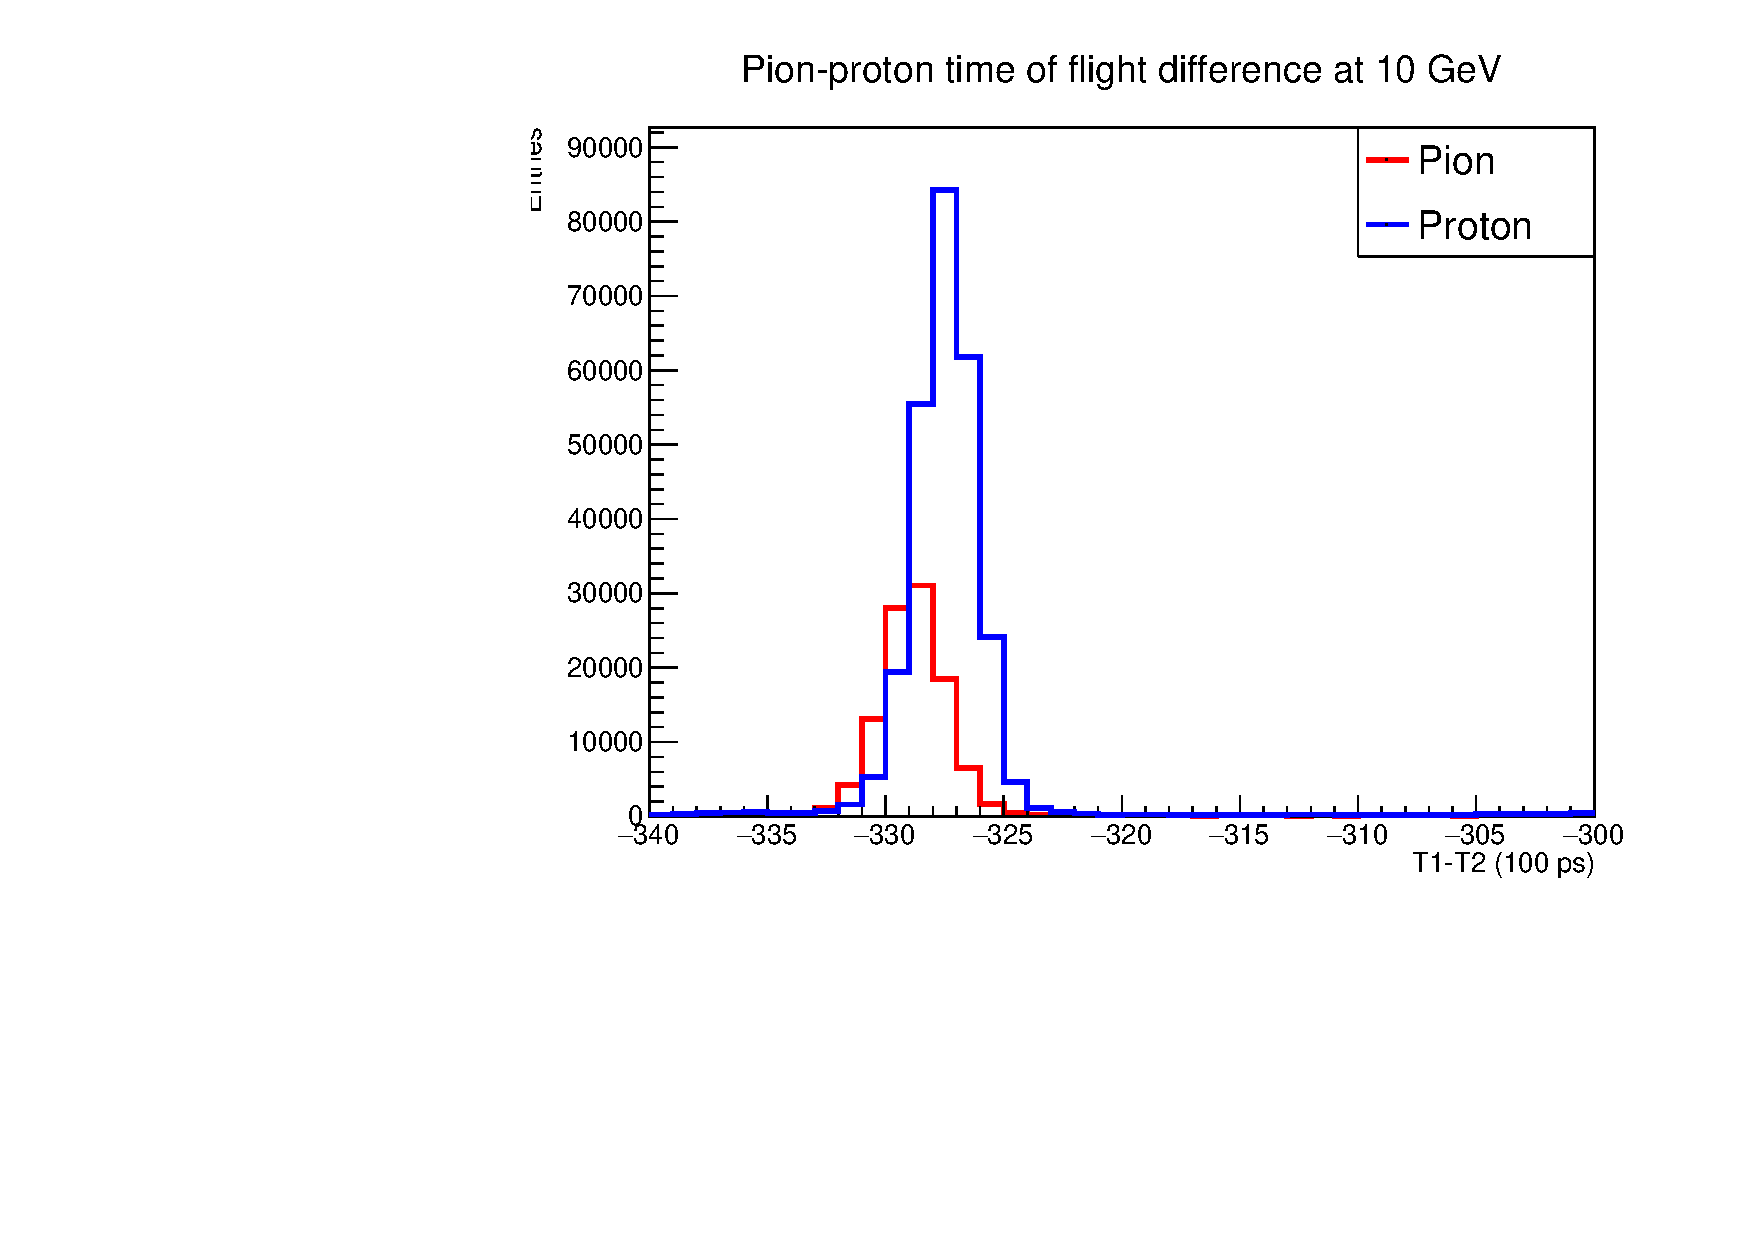
\includegraphics[width = 0.7\textwidth]{Figs/PionProton_TimeDiff_10GeV.pdf}
  \end{figure}
\end{frame}

\begin{frame}{2022 test beam analysis}
  \begin{center}
    \Large{Let's look at hit maps of $\SI{3}{\giga\eV/c}$ pions...}
  \end{center}
  \begin{figure}
    \centering
    \begin{subfigure}{0.5\textwidth}
      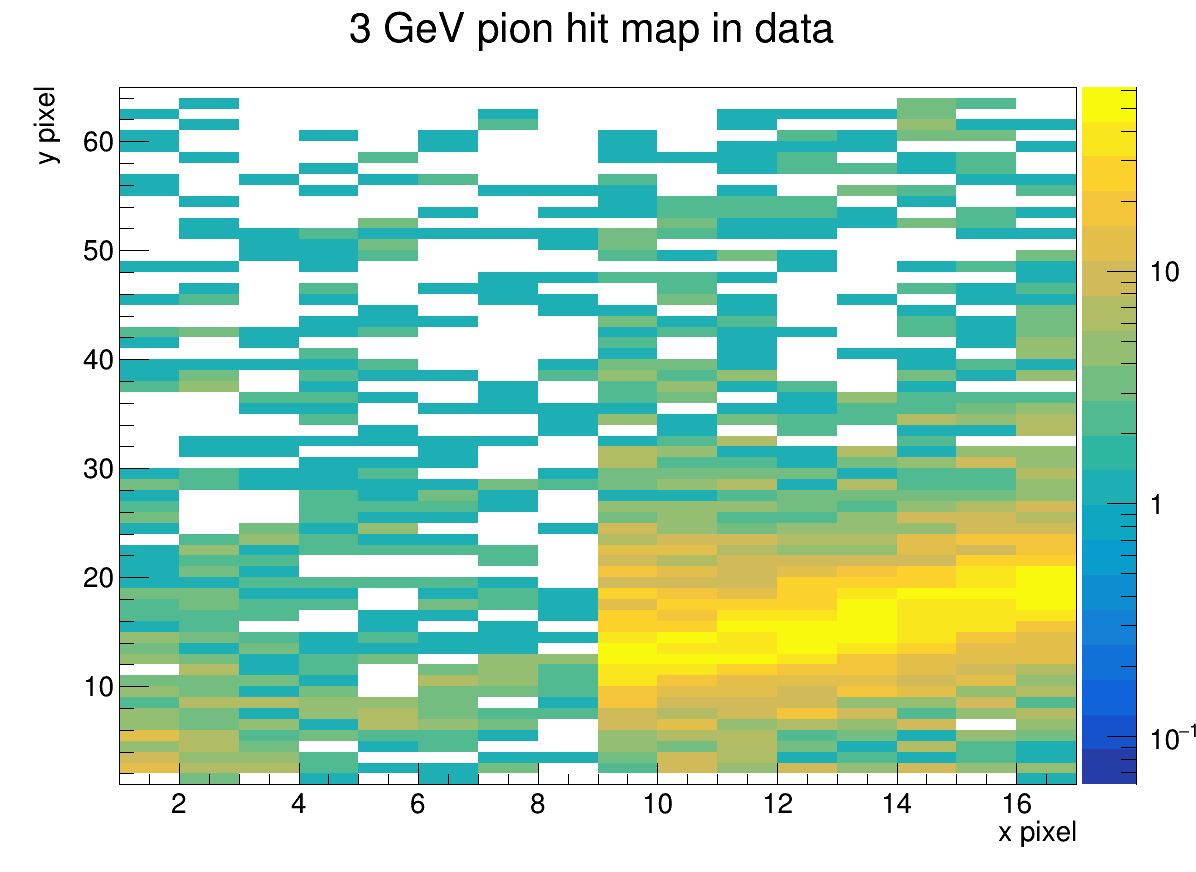
\includegraphics[width = 1.0\textwidth]{Figs/HitMap_Pos8_Pion_3GeV_Data.png}
      \caption{Testbeam data}
    \end{subfigure}%
    \begin{subfigure}{0.5\textwidth}
      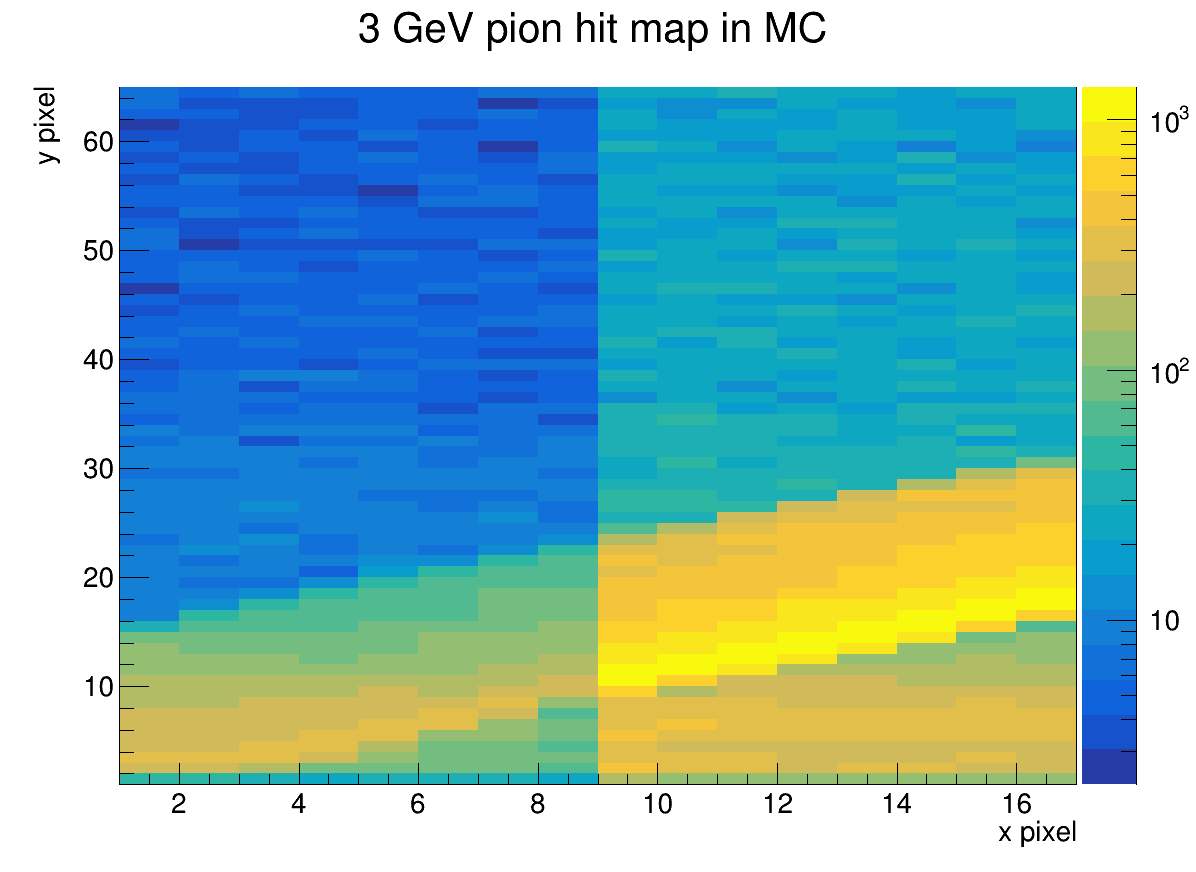
\includegraphics[width = 1.0\textwidth]{Figs/HitMap_Pos8_Pion_3GeV_MC.png}
      \caption{Geant4 simulation}
    \end{subfigure}%
  \end{figure}
\end{frame}

\begin{frame}{2022 test beam analysis}
  \begin{center}
    \Large{... and compare with hit maps of $\SI{3}{\giga\eV/c}$ protons}
  \end{center}
  \begin{figure}
    \centering
    \begin{subfigure}{0.5\textwidth}
      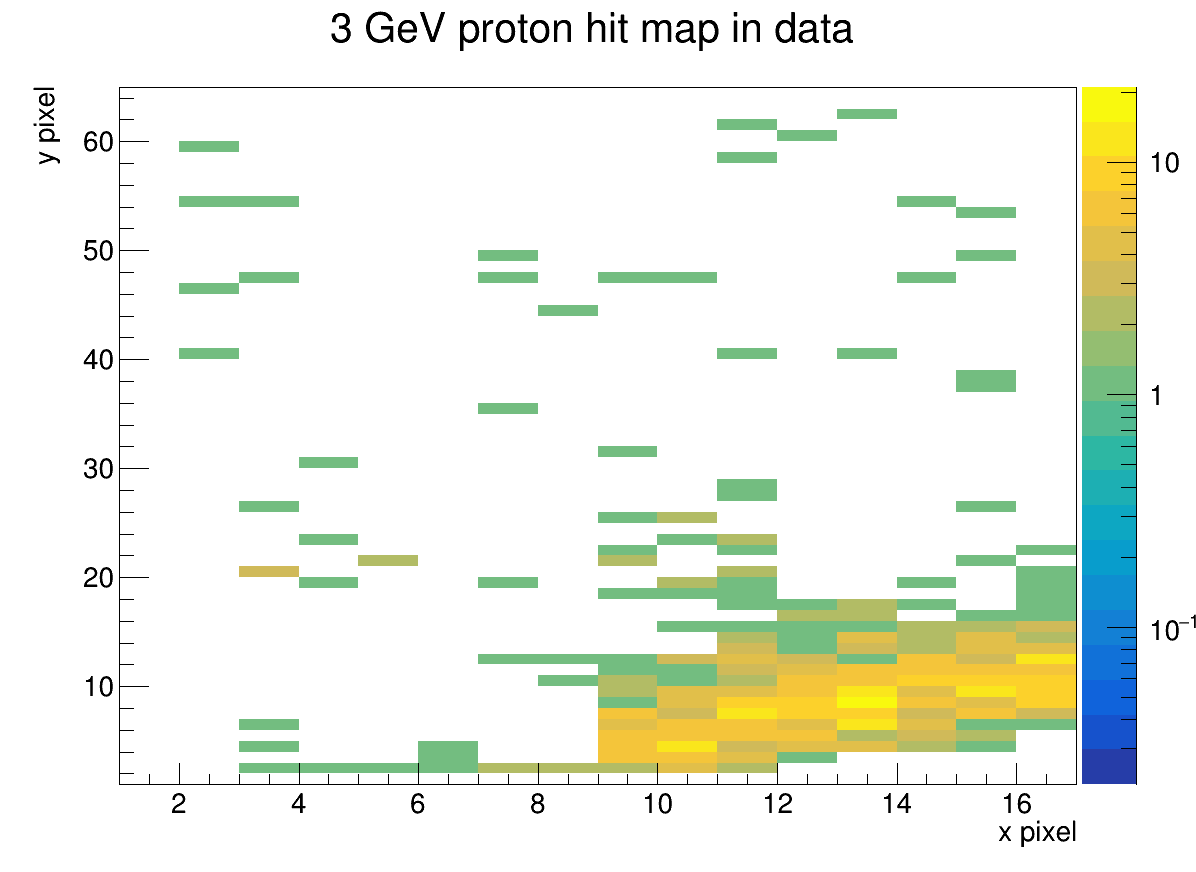
\includegraphics[width = 1.0\textwidth]{Figs/HitMap_Pos8_Proton_3GeV_Data.png}
      \caption{Testbeam data}
    \end{subfigure}%
    \begin{subfigure}{0.5\textwidth}
      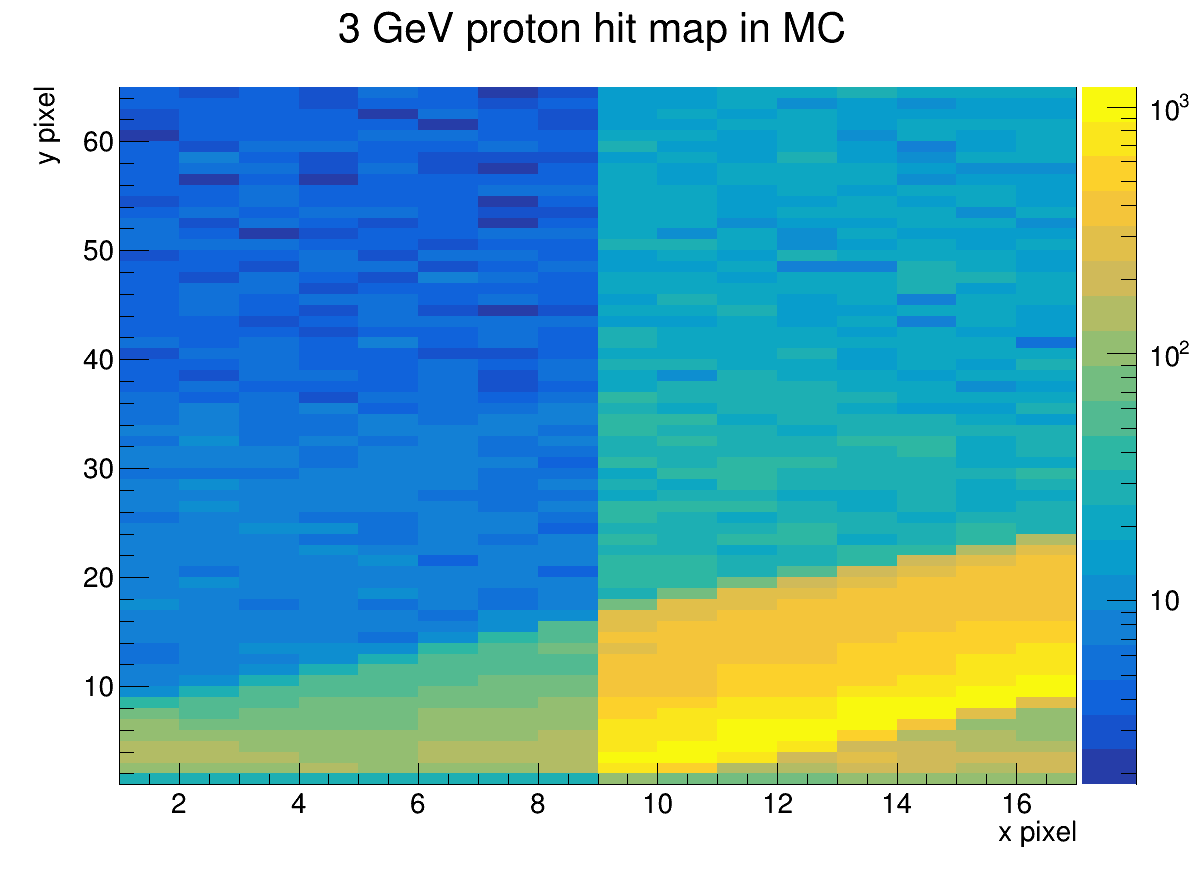
\includegraphics[width = 1.0\textwidth]{Figs/HitMap_Pos8_Proton_3GeV_MC.png}
      \caption{Geant4 simulation}
    \end{subfigure}%
  \end{figure}
\end{frame}

\begin{frame}{2022 test beam analysis}
  \begin{center}
    \Large{Different y-position $\implies$ Separation in Cherenkov angle}
  \end{center}
  \begin{figure}
    \centering
    \begin{subfigure}{0.5\textwidth}
      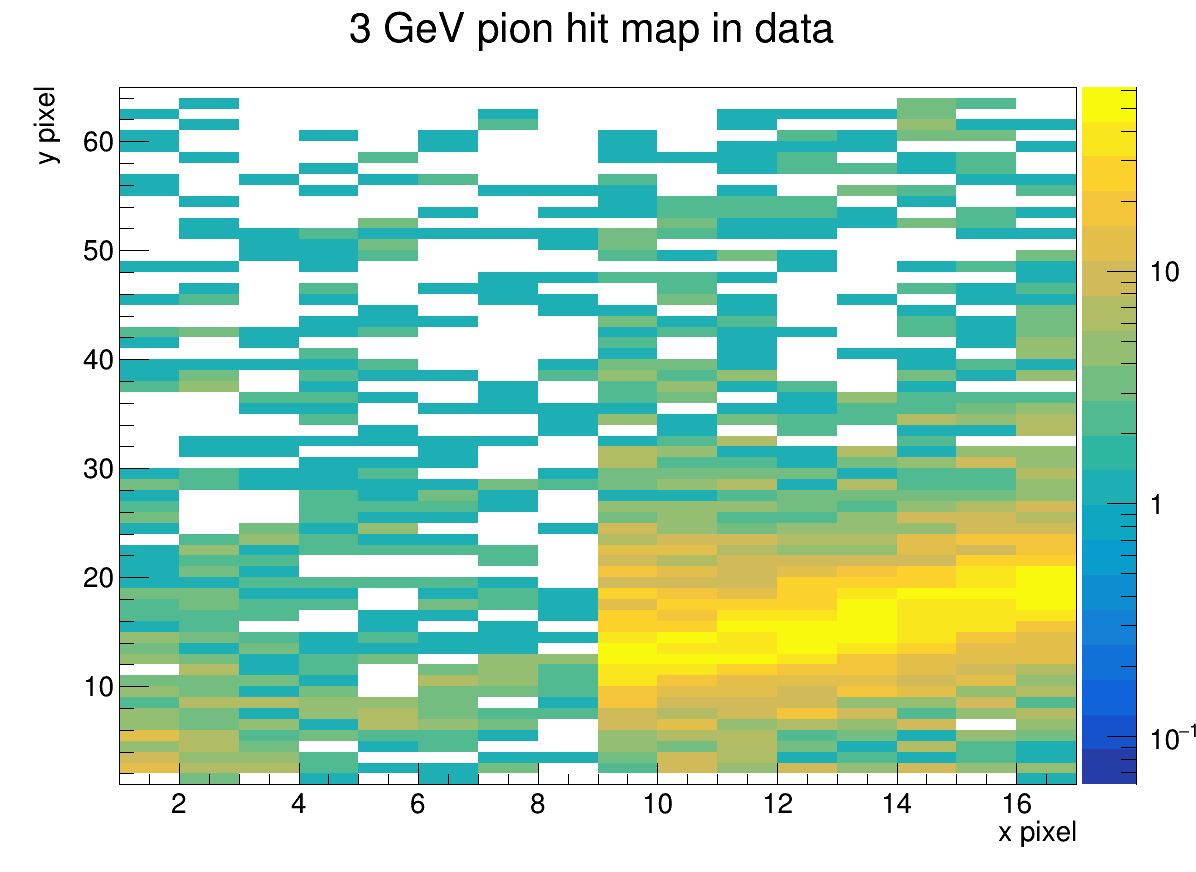
\includegraphics[width = 1.0\textwidth]{Figs/HitMap_Pos8_Pion_3GeV_Data.png}
      \caption{Pions}
    \end{subfigure}%
    \begin{subfigure}{0.5\textwidth}
      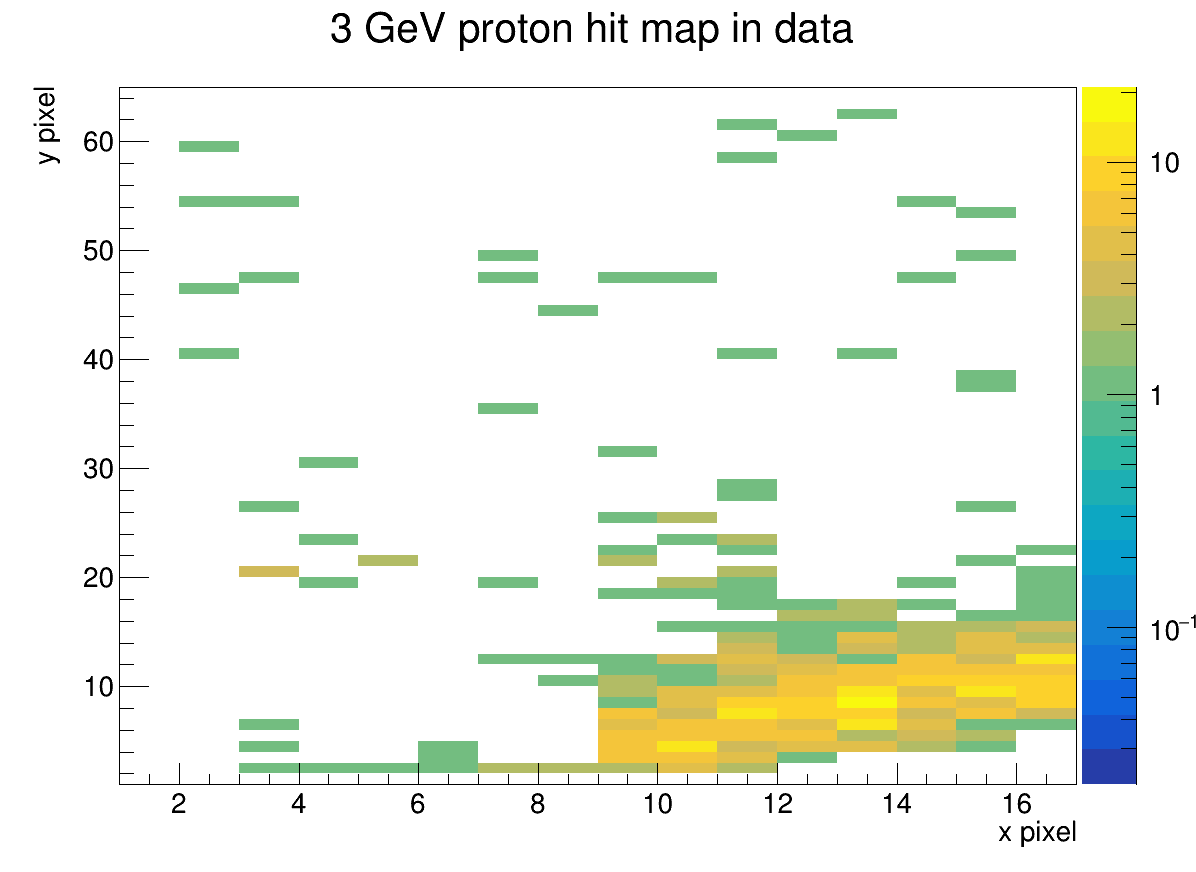
\includegraphics[width = 1.0\textwidth]{Figs/HitMap_Pos8_Proton_3GeV_Data.png}
      \caption{Protons}
    \end{subfigure}%
  \end{figure}
\end{frame}

\begin{frame}{2022 test beam analysis}
  \begin{center}
    \Large{What about timing information? First look at $\SI{10}{\giga\eV/c}$ pions and protons}
  \end{center}
  \begin{figure}
    \centering
    \begin{subfigure}{0.5\textwidth}
      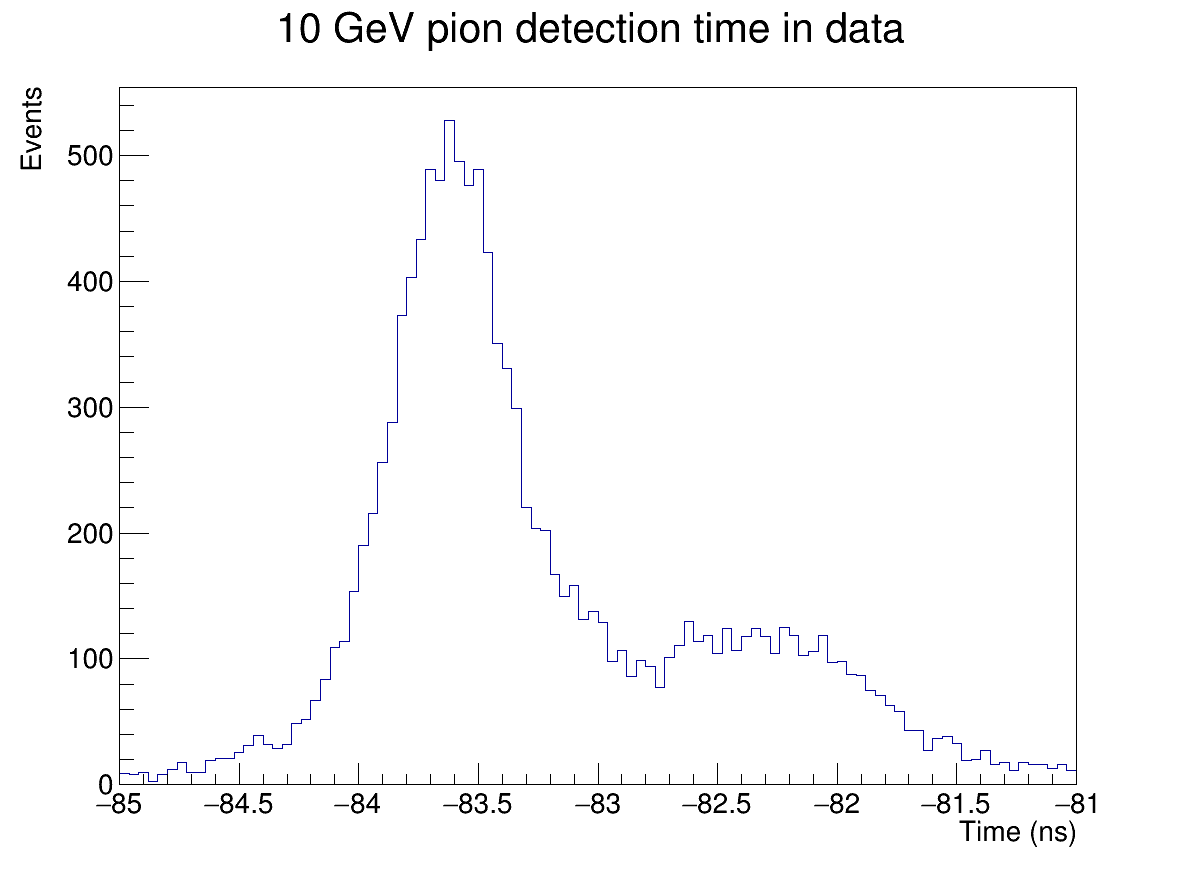
\includegraphics[width = 1.0\textwidth]{Figs/Time_Pos8_Pion_10GeV_Data.png}
      \caption{Pions}
    \end{subfigure}%
    \begin{subfigure}{0.5\textwidth}
      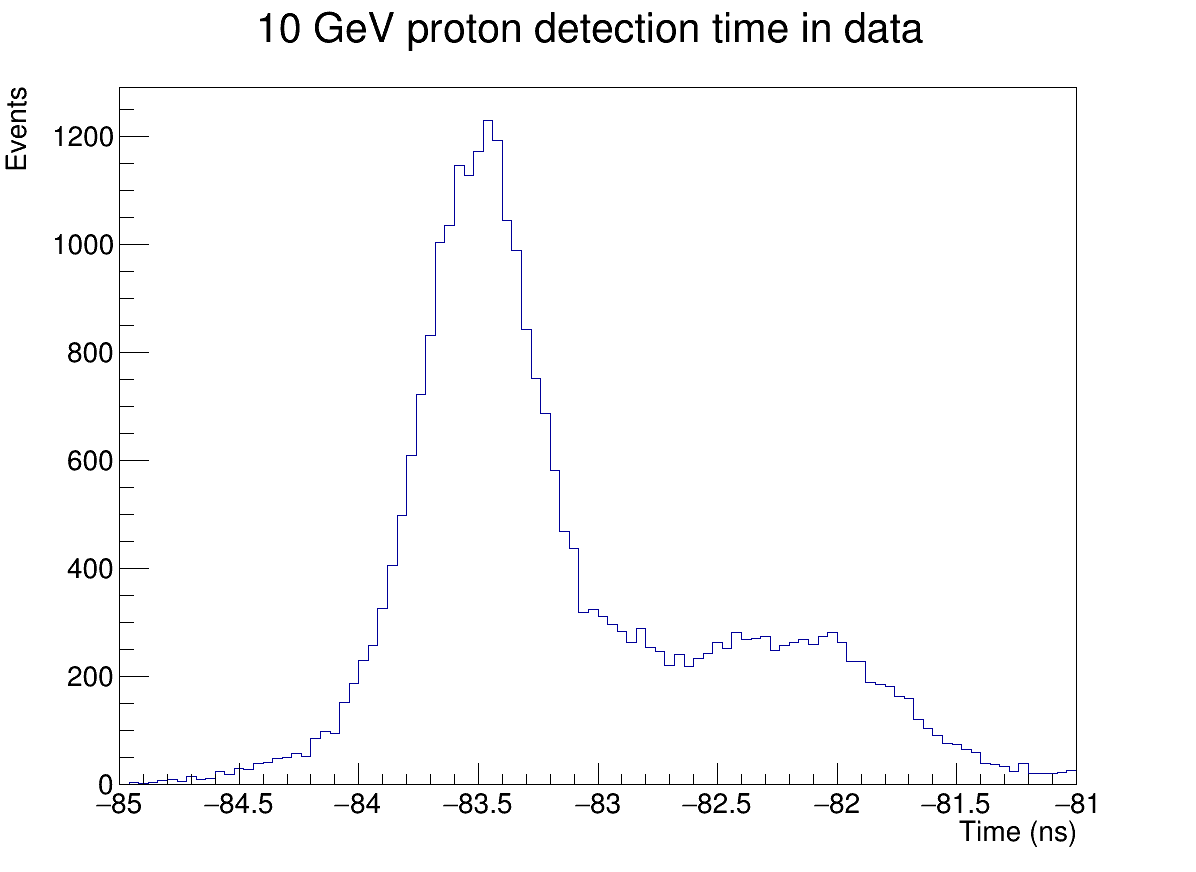
\includegraphics[width = 1.0\textwidth]{Figs/Time_Pos8_Proton_10GeV_Data.png}
      \caption{Protons}
    \end{subfigure}%
  \end{figure}
  \begin{center}
    Small ($\SI{0.15}{\nano\second}$) separation, as expected
  \end{center}
\end{frame}

\begin{frame}{2022 test beam analysis}
  \begin{center}
    \Large{What about timing information? First look at $\SI{10}{\giga\eV}$ pions and protons}
  \end{center}
  \begin{figure}
    \centering
    \begin{subfigure}{0.5\textwidth}
      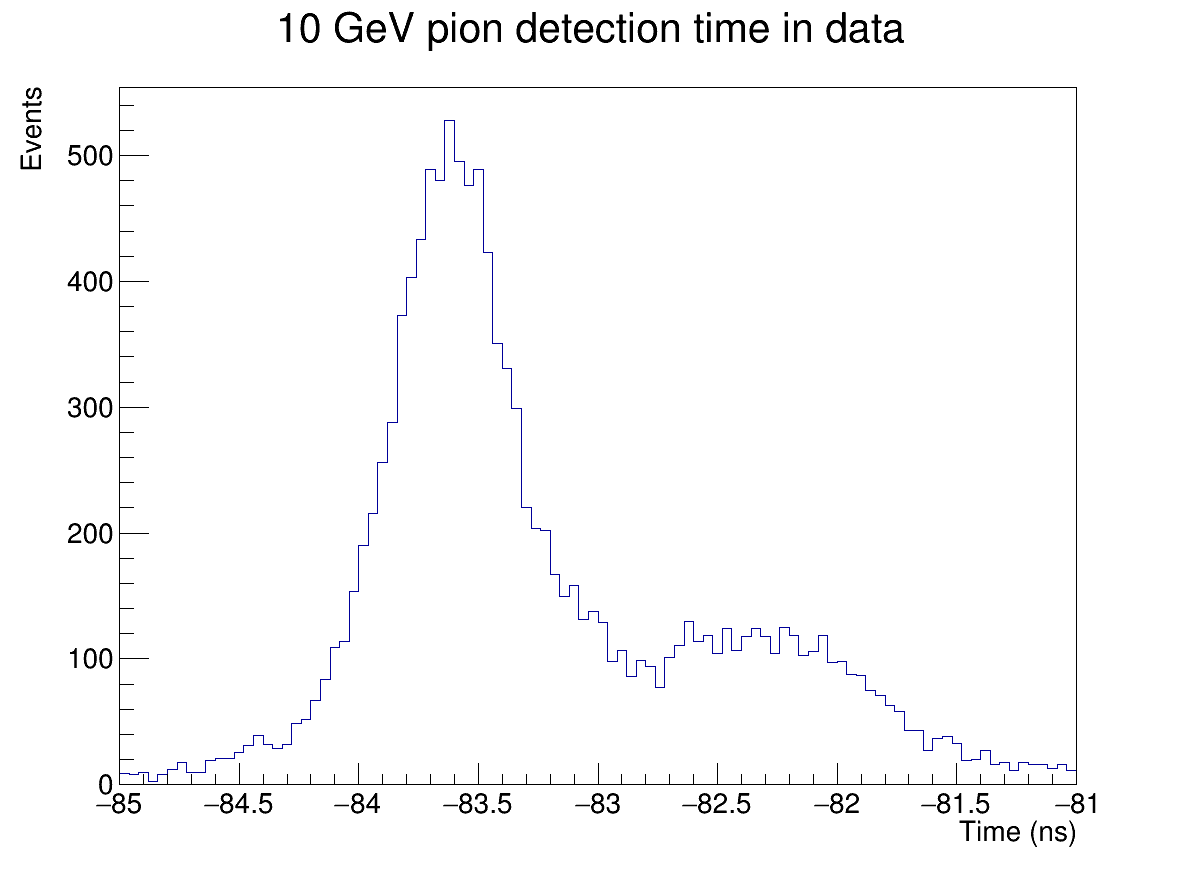
\includegraphics[width = 1.0\textwidth]{Figs/Time_Pos8_Pion_10GeV_Data.png}
      \caption{Pions}
    \end{subfigure}%
    \begin{subfigure}{0.5\textwidth}
      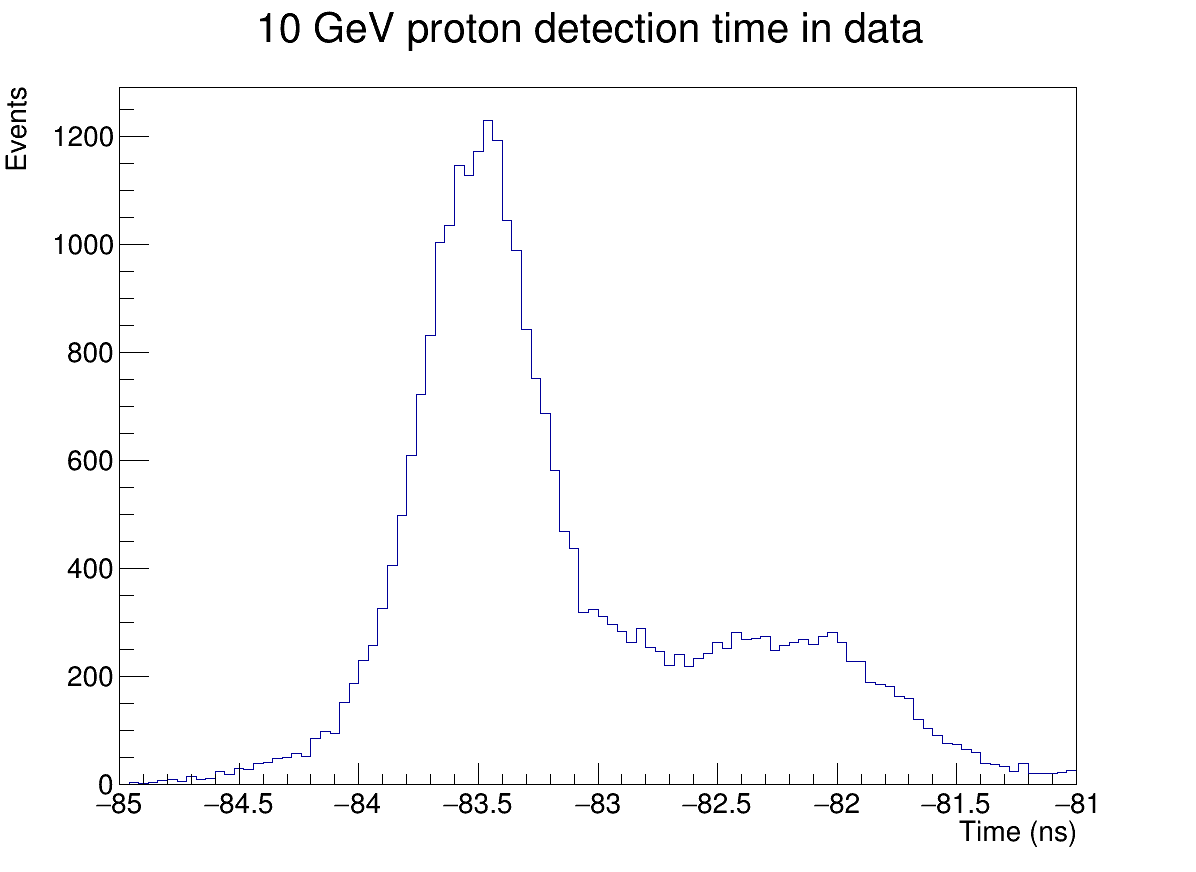
\includegraphics[width = 1.0\textwidth]{Figs/Time_Pos8_Proton_10GeV_Data.png}
      \caption{Protons}
    \end{subfigure}%
  \end{figure}
  \begin{center}
    Additional ``reflection'', which arrives $\sim\SI{1}{\nano\second}$ later, is currently under study\phantom{(}
  \end{center}
\end{frame}

\begin{frame}{2022 test beam analysis}
  \begin{center}
    \Large{Then consider the $\SI{3}{\giga\eV/c}$ pions and protons, where a clear separation in arrival time is seen}
  \end{center}
  \begin{figure}
    \centering
    \begin{subfigure}{0.5\textwidth}
      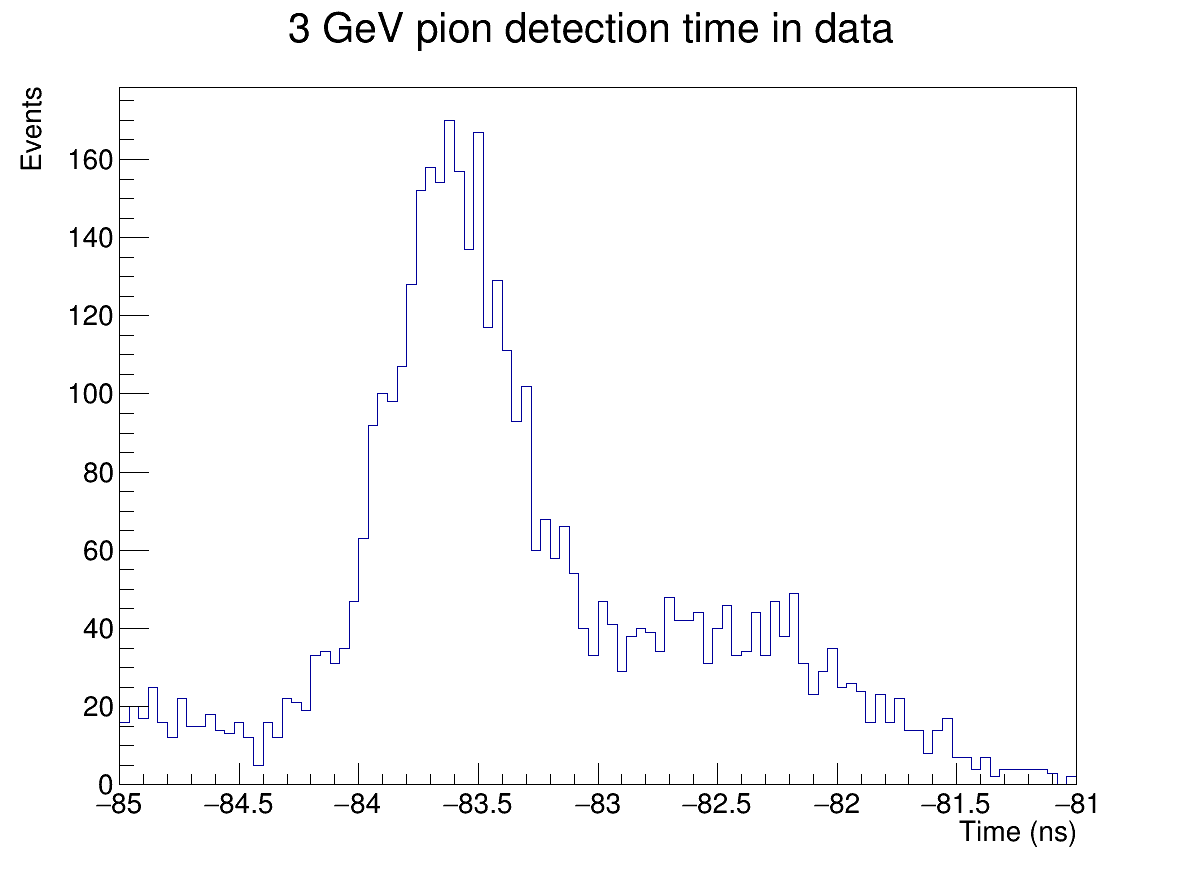
\includegraphics[width = 1.0\textwidth]{Figs/Time_Pos8_Pion_3GeV_Data.png}
      \caption{Pions}
    \end{subfigure}%
    \begin{subfigure}{0.5\textwidth}
      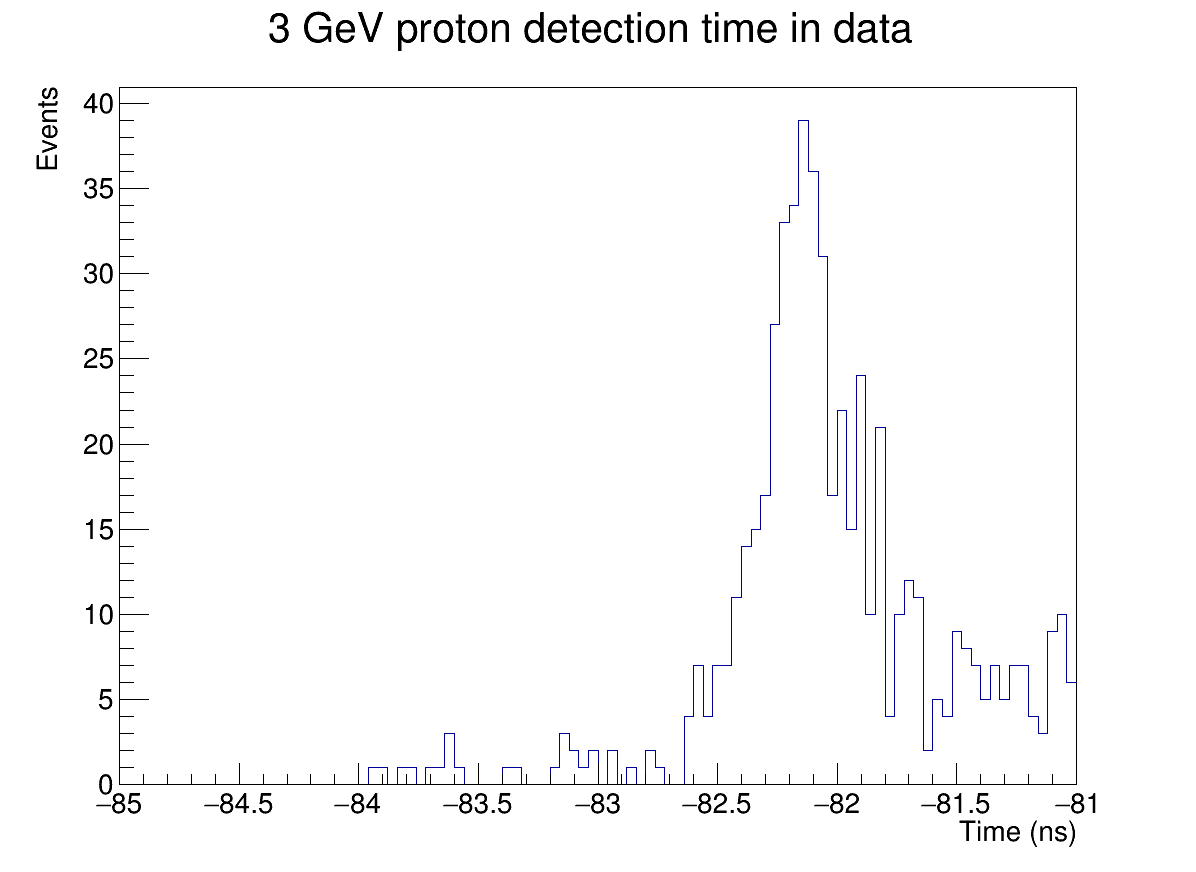
\includegraphics[width = 1.0\textwidth]{Figs/Time_Pos8_Proton_3GeV_Data.png}
      \caption{Protons}
    \end{subfigure}%
  \end{figure}
  \begin{center}
    Additional reflection also arrives later for protons\phantom{(}
  \end{center}
\end{frame}

\begin{frame}{PID algorithm}
  \begin{itemize}
    \setlength\itemsep{1.0em}
    \item{Long term goal: Demonstrate separation between pions and protons using a PID algorithm}
    \item{PID algorithm presented by \href{https://indico.cern.ch/event/1204659/timetable/\#21-wp3-torch-reconstruction}{Tom Jones} last year:}
  \end{itemize}
  \vspace{0.4cm}
  \begin{equation*}
    P(E_\gamma, \phi_c, t_0) = P(E_\gamma)\times P(\phi_c)\times P(t_0)
  \end{equation*}
  \begin{enumerate}
    \setlength\itemsep{1.0em}
    \item{$P(E_\gamma)$: Frank-Tamm distribution $\circledast$ Efficiency effects}
    \item{$P(\phi_c)$: Uniform distribution}
    \item{$P(t_0)$: Gaussian smearing due to electronics and photon reconstruction (pixel size and emission point assumptions)}
  \end{enumerate}
\end{frame}

\begin{frame}{PID algorithm}
  \begin{itemize}
    \setlength\itemsep{1.0em}
    \item{Long term goal: Demonstrate separation between pions and protons using a PID algorithm}
    \item{PID algorithm presented by \href{https://indico.cern.ch/event/1204659/timetable/\#21-wp3-torch-reconstruction}{Tom Jones} last year:}
  \end{itemize}
  \vspace{0.4cm}
  \begin{equation*}
    P(E_\gamma, \phi_c, t_0) = P(E_\gamma)\times P(\phi_c)\times P(t_0)
  \end{equation*}
  \vspace{-0.39cm}
  \begin{itemize}
    \setlength\itemsep{1.0em}
    \item{Convert $(E_\gamma, \phi_c)$ into detector hit position $(x, y)$ using Jacobian $J$}
    \item{Each derivative in $J$ is calculated by forward-propagating two photons}
    \item{Integrate over each pixel using 2D trapezium rule}
  \end{itemize}
  \vspace{0.4cm}
  \begin{equation*}
    P(x, y, t_0) = P(E_\gamma, \phi_c, t_0)/\lvert J\rvert
  \end{equation*}
  \vspace{-0.63cm}
\end{frame}

\section{Future plans}

\begin{frame}{Future plans: Testbeam in 2025}
  \begin{center}
    {\Large 2025 testbeam}
  \end{center}
  \begin{itemize}
    \setlength\itemsep{1.0em}
    \item{The TORCH collaboration is planning on going back to T9 in early 2025 with a $\SI{2.5}{\meter}$ length prototype TORCH module}
    \item{Completely new mechanical support structure, which will be discussed by Adam in the next talk!}
    \item{From our experience with the 2022 testbeam, we will be much better prepared for 2025:}
    \begin{itemize}
      \item{More efficient data collection}
      \item{Better quality data}
      \item{First demonstration with full-size prototype}
    \end{itemize}
  \end{itemize}
\end{frame}

\begin{frame}{Future plans: New electronics}
  \begin{itemize}
    \setlength\itemsep{0.7em}
    \item{New electronics: FastIC $+$ PicoTDC $+$ lpGBT developed by RICH}
    \begin{itemize}
      \item{Only 2 sets available, which is insufficient for the next testbeam}
      \item{Expected delivery at beginning of 2024}
    \end{itemize}
    \item{FastIC chips will replace old NINO chips}
    \begin{itemize}
      \item{$\SI{250}{\nano\meter}\to\SI{65}{\nano\meter}$ CMOS technology}
    \end{itemize}
    \item{PicoTDC replace previous HPTDC chips}
    \begin{itemize}
      \item{Time binning is improved from $\SI{100}{\pico\second}$ to $\SI{12}{\pico\second}$}
      \item{In the longer term, plan to use the FastRICH chip}
    \end{itemize}
    \item{Testing with RICH carrier board and TORCH specific adaptor board}
  \end{itemize}
  \begin{figure}
    \centering
    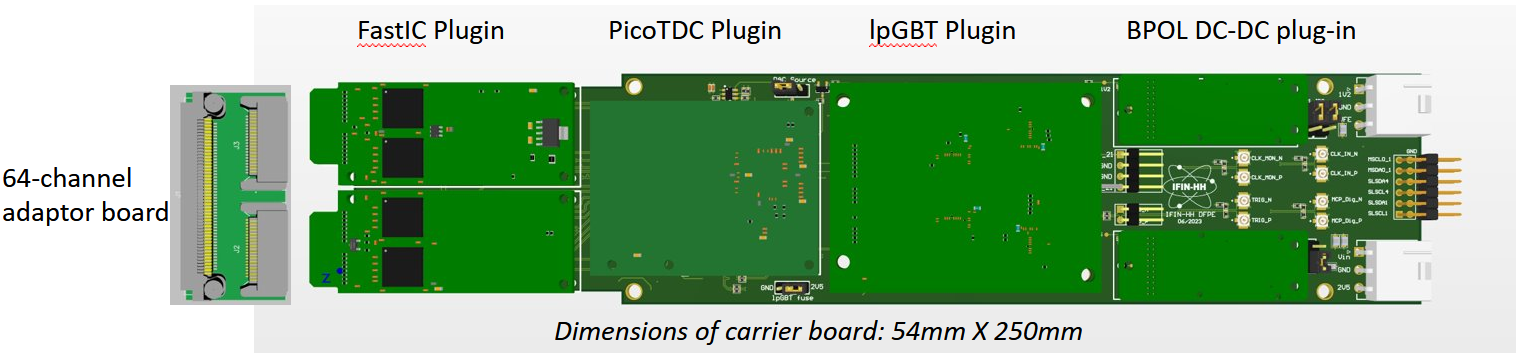
\includegraphics[width = 1.0\textwidth]{Figs/NewTORCHElectronics.png}
  \end{figure}
\end{frame}

\begin{frame}{Future plans: New MCP-PMT tubes}
  \begin{columns}
    \begin{column}{0.58\textwidth}
      \begin{itemize}
        \setlength\itemsep{1.0em}
        \item{Working with commerical partner, Photek Ltd, to develop MCP-PMTs suitable for HL-LHC}
        \item{From FTDR studies, we know centre module occupancy must be improved}
        \item{Increase granularity: $8\times 64\to 16\times 96$}
        \item{AC coupled $\to$ DC coupled anode}
      \end{itemize}
      \vspace{0.0cm}
      \begin{figure}
        \centering
        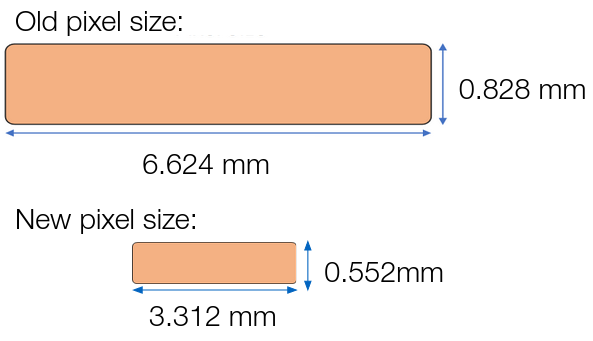
\includegraphics[width = 0.68\textwidth]{Figs/NewMCPSizeComparison.png}
      \end{figure}
    \end{column}
    \begin{column}{0.42\textwidth}
      \begin{figure}
        \centering
        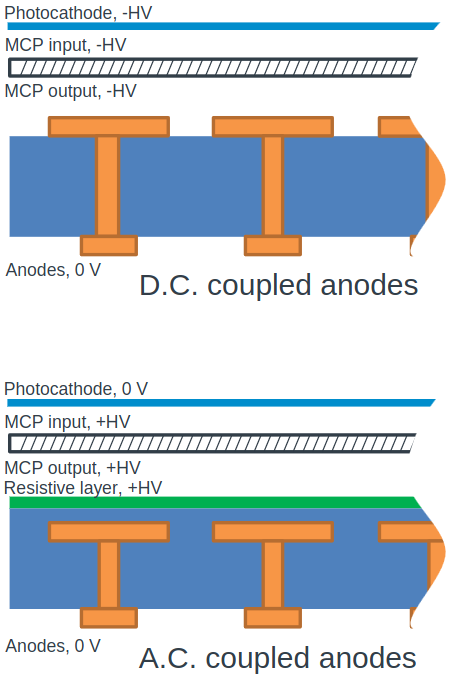
\includegraphics[width = 0.9\textwidth]{Figs/ACvsDCCoupledAnode.png}
      \end{figure}
    \end{column}
  \end{columns}
\end{frame}

\begin{frame}{Future plans: New MCP-PMT tubes}
  \begin{columns}
    \begin{column}{0.5\textwidth}
      \begin{itemize}
        \setlength\itemsep{1.0em}
        \item{New MCP-PMT has a ceramic anode with vias to route the signal to connectors on the back}
        \item{Connectors will be soldered with laser-jet soldering:}
        \begin{itemize}
          \item{Required by the density of the readout}
          \item{Needed to avoid heating the tube}
        \end{itemize}
        \item{Expect delivery at end of February}
      \end{itemize}
    \end{column}
    \begin{column}{0.5\textwidth}
      \begin{figure}
        \centering
        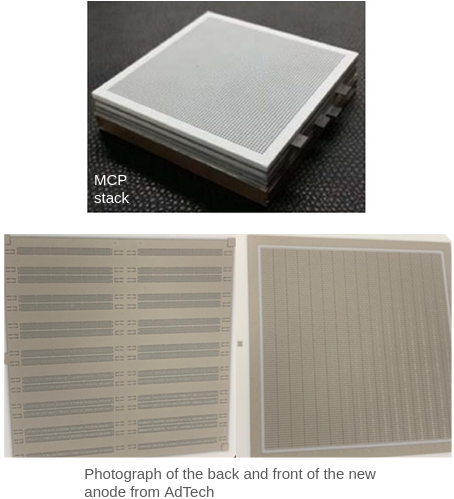
\includegraphics[width = 0.9\textwidth]{Figs/NewMCPFrontBack.png}
      \end{figure}
    \end{column}
  \end{columns}
\end{frame}

\begin{frame}{Future plans: Lab testing of new MCP-PMT tubes}
  \begin{figure}
    \centering
    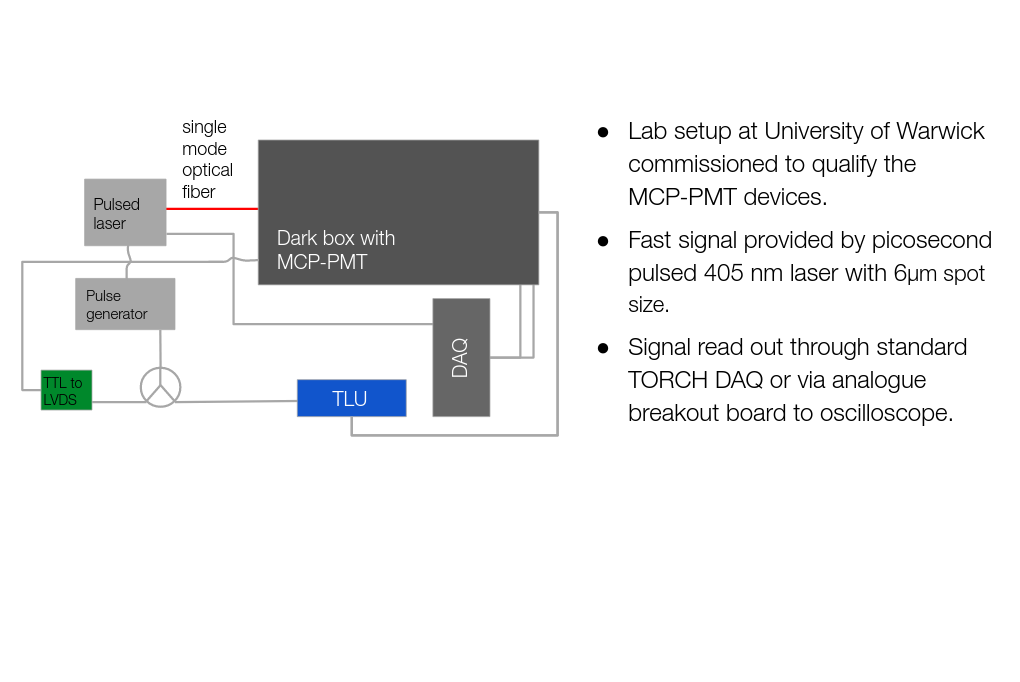
\includegraphics[width = 0.95\textwidth]{Figs/WarwickLabSetup.png}
  \end{figure}
\end{frame}

\begin{frame}{Future plans: Lab testing of new MCP-PMT tubes}
  \begin{figure}
    \centering
    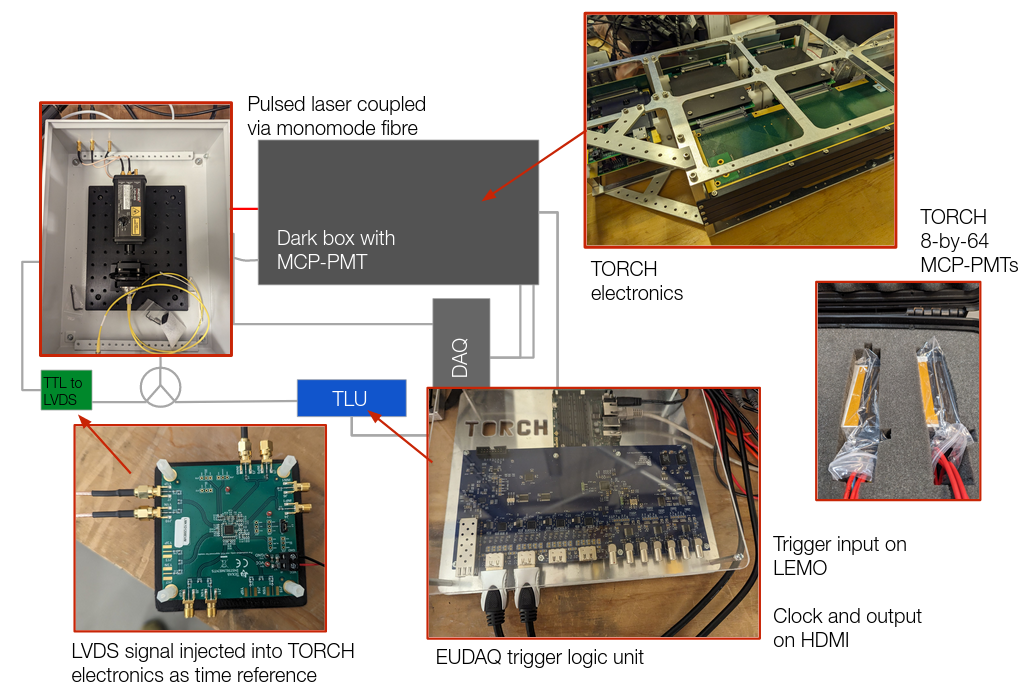
\includegraphics[width = 0.95\textwidth]{Figs/WarwickLabSetupPhotos.png}
  \end{figure}
\end{frame}

\section{Summary and future prospects}

\begin{frame}{Summary and future prospects}
  \vspace{0.3cm}
  {\Large Summary:}
  \vspace{0.5cm}
  \begin{enumerate}
    \setlength\itemsep{1.5em}
    \item{Test beam analysis progressing well}
    \begin{itemize}
      \item{Hit patterns well understood}
      \item{More detailed analysis of time information ongoing}
      \item{Improved calibration is essential}
    \end{itemize}
    \item{We are acquiring new electronics and new MCP-PMTs}
    \begin{itemize}
      \item{Lab testing of electronics ongoing}
      \item{New electronics will replace legacy NINOs and HPTDCs}
      \item{New MCP-MPTs have higher spatial resolution}
      \item{Delivery of new MCP-PMT tubes expected at the end of February}
    \end{itemize}
  \end{enumerate}
\end{frame}

\begin{frame}{Summary and future prospects}
  \vspace{0.3cm}
  {\Large Future prospects:}
  \vspace{0.5cm}
  \begin{enumerate}
    \setlength\itemsep{1.5em}
    \item{Finalise test beam analysis}
    \begin{itemize}
      \item{Calibrations}
      \item{Photon counting}
      \item{Time resolution}
      \item{PID performance}
    \end{itemize}
    \item{New test beam is planned for early 2025}
    \begin{itemize}
      \item{Demonstration of full height quartz plate TORCH and mechanics}
    \end{itemize}
  \end{enumerate}
  \vspace{0.5cm}
  \begin{center}
    {\huge Thanks for your attention!}
  \end{center}
\end{frame}

\begin{frame}{Backup slides}
  \begin{center}
    {\huge Backup slides}
  \end{center}
\end{frame}

\begin{frame}{Backup: Reminder of Photek MCP-PMT}
  \begin{itemize}
    \setlength\itemsep{0.7em}
    \item{Photon detector: MicroChannel Plate PhotoMultiplier Tube}
    \begin{itemize}
      \item[-]{T.M. Conneely \textit{et al} 2016 \textit{JINST} \textbf{10} C05003}
    \end{itemize}
    \item{$53\times 53\si{\milli\meter\squared}$ active area}
    \item{$8$ columns, each with $64$ pixels}
    \item{Effectively $128$ pixels with charge sharing}
  \end{itemize}
  \vspace{-0.35cm}
  \begin{figure}
    \centering
    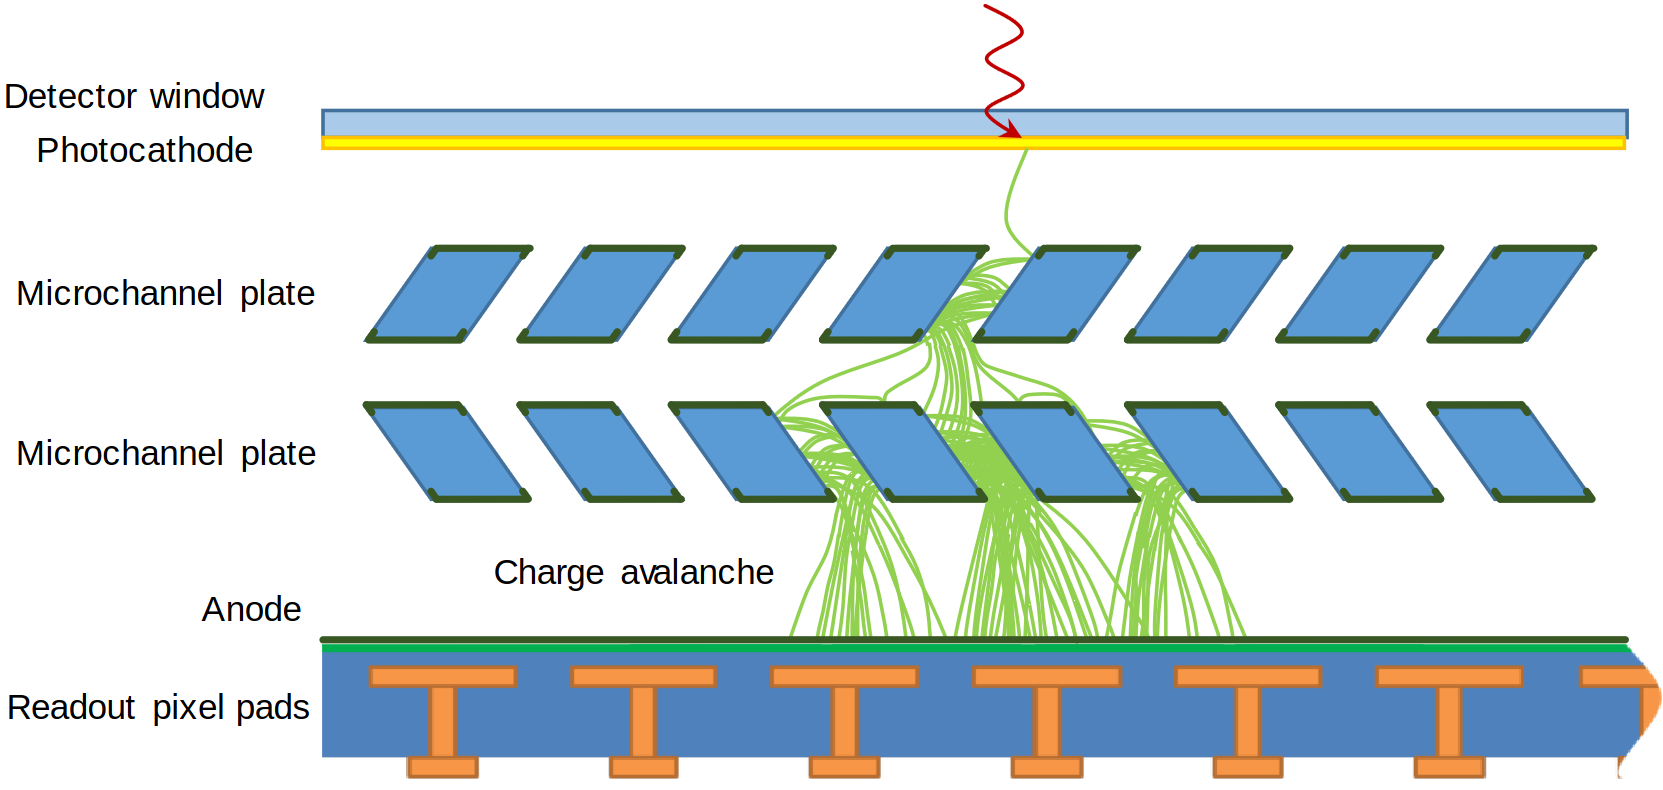
\includegraphics[width = 0.8\textwidth]{Figs/MCP_PMT_illustration.png}
  \end{figure}
\end{frame}

\begin{frame}{Backup: TORCH electronics}
  \begin{itemize}
    \setlength\itemsep{0.7em}
    \item{NINO: Amplifier and discriminator}
    \begin{itemize}
      \item[-]{R. Gao \textit{et al} 2022 \textit{JINST} \textbf{17} C05015}
    \end{itemize}
    \item{High Performance Time to Digital Converter: $\SI{100}{\pico\second}$ bins}
    \item{Legacy electronics that will be replaced, more on this later!}
  \end{itemize}
  \begin{figure}
    \centering
    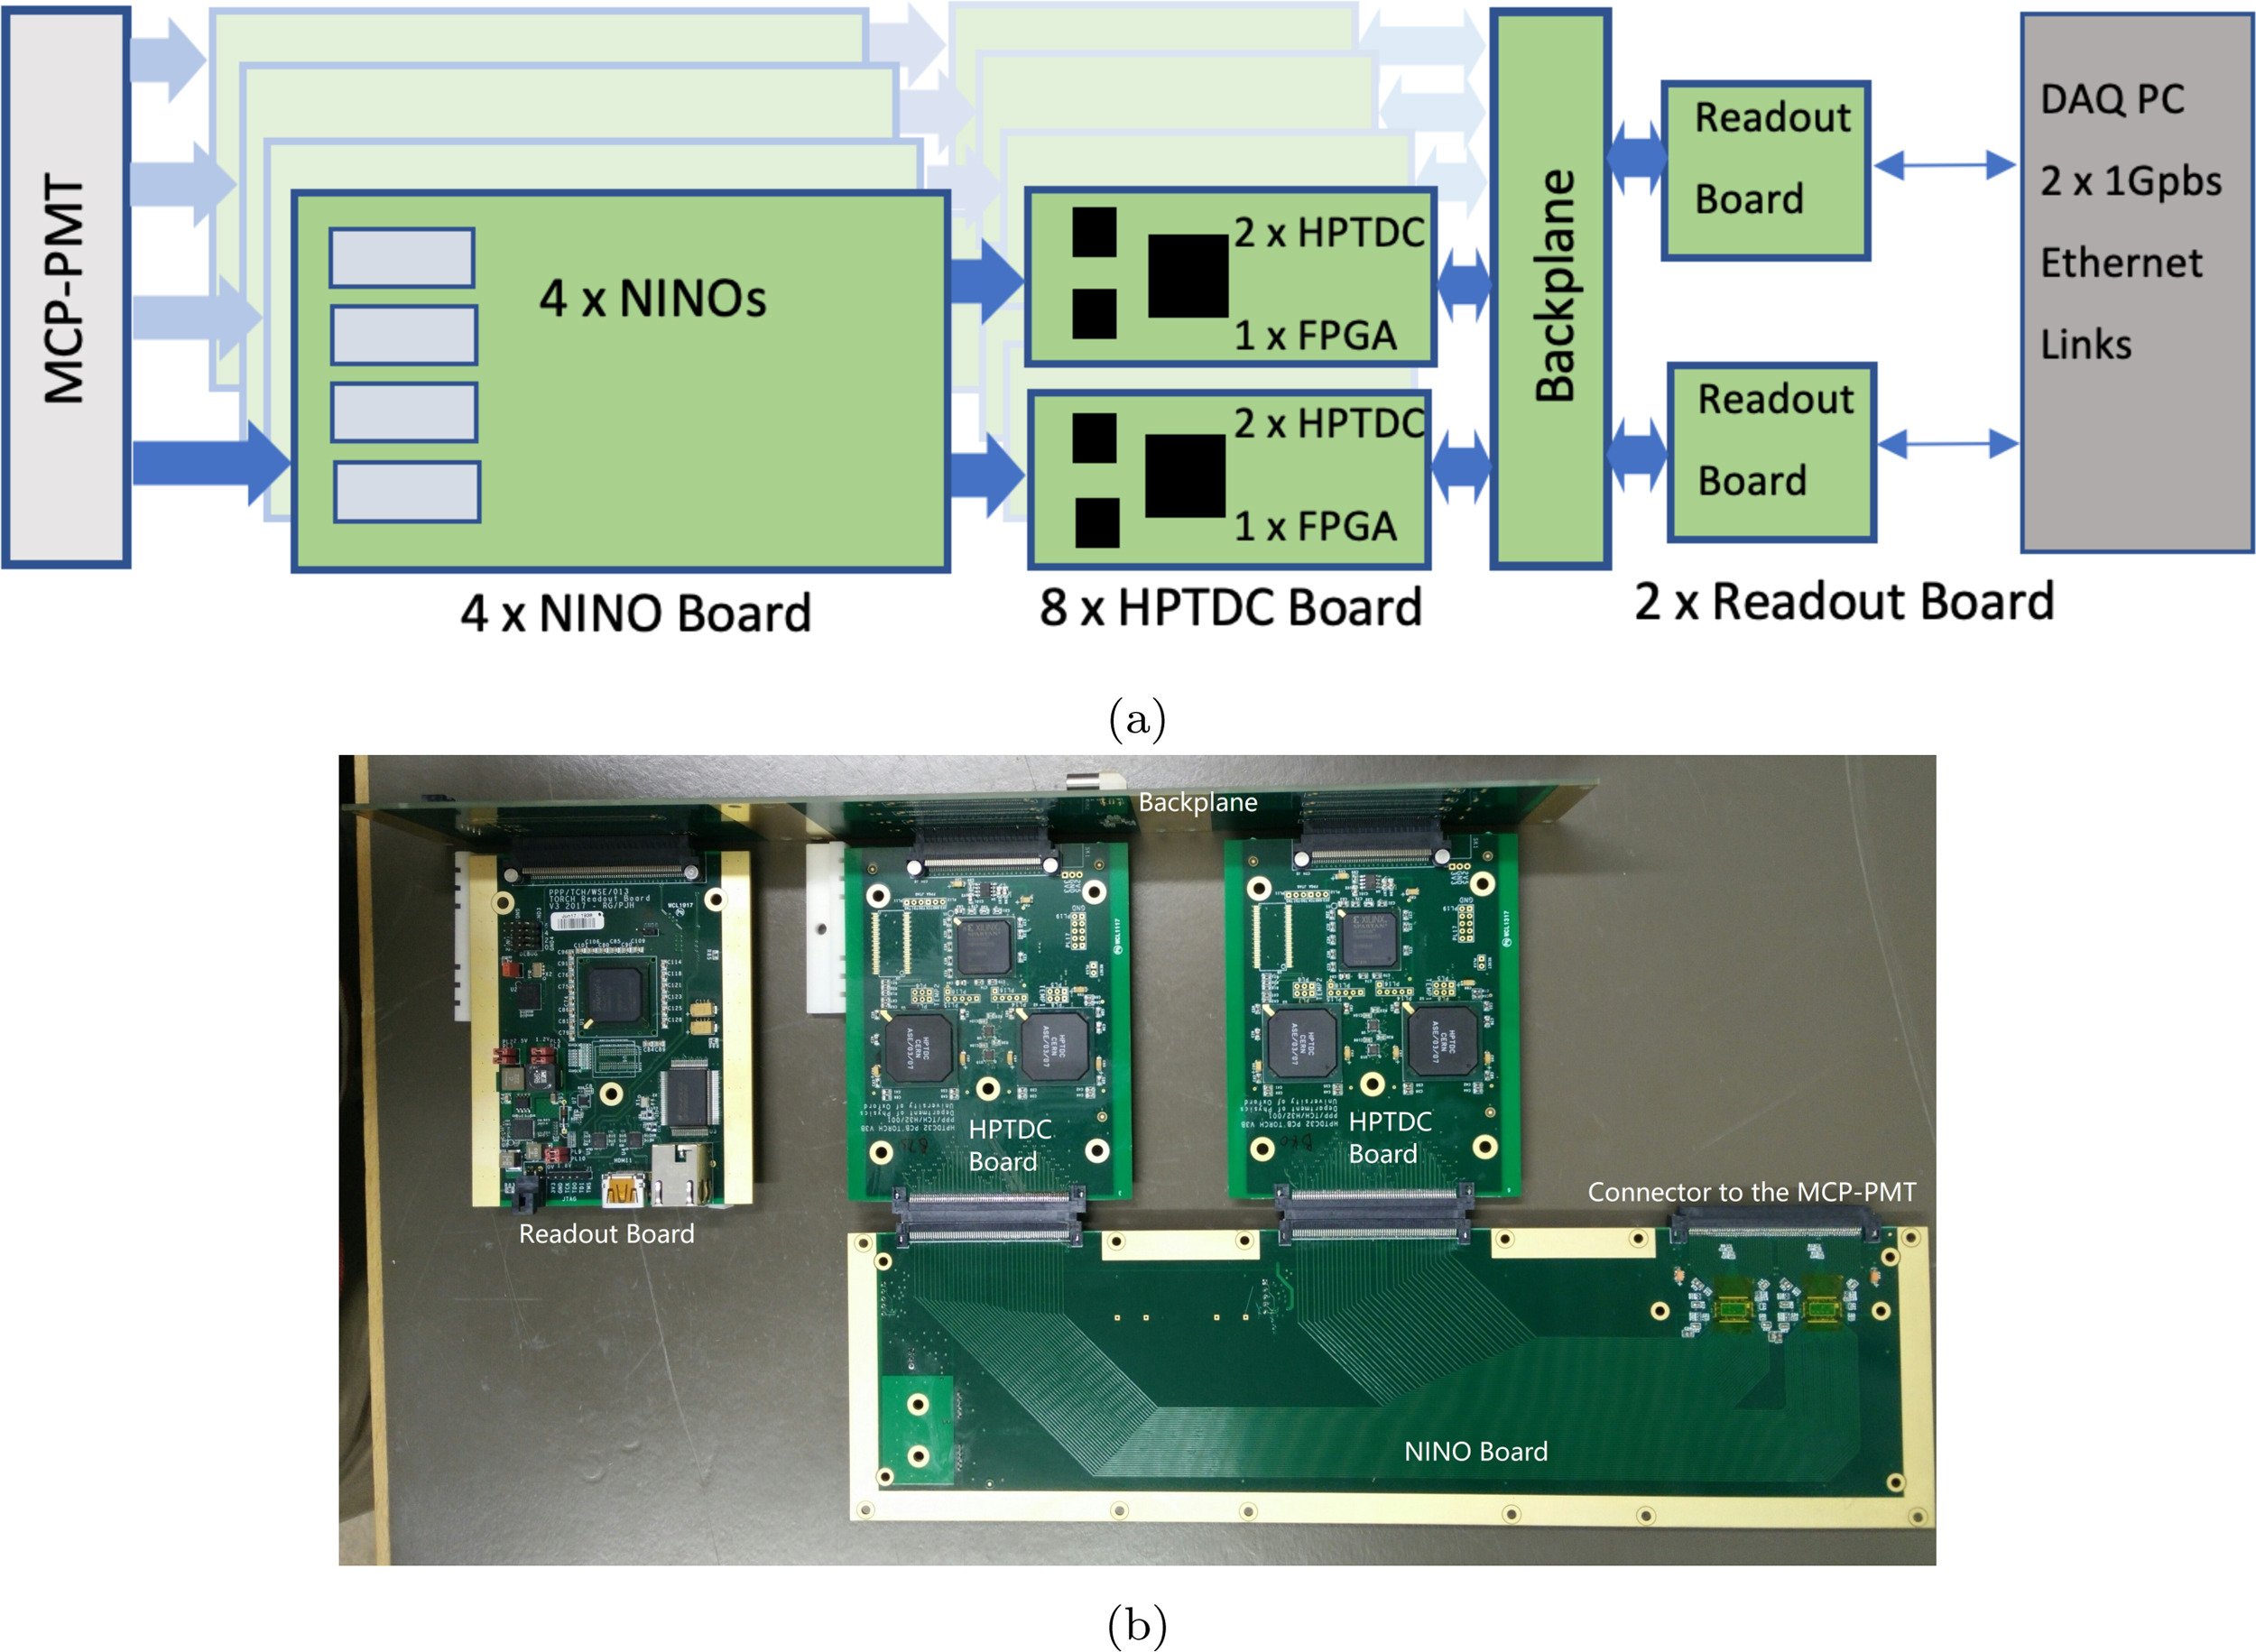
\includegraphics[width = 1.0\textwidth,trim={0 0.3cm 0 4.2cm},clip=true]{Figs/TORCH_testbeam_2018_electronics.jpg}
  \end{figure}
\end{frame}

\end{document}
